% options:
% thesis=B bachelor's thesis
% thesis=M master's thesis
% czech thesis in Czech language
% english thesis in English language
% hidelinks remove colour boxes around hyperlinks

\documentclass[thesis=B,czech]{FITthesis}[2013/10/20]

\usepackage[utf8]{inputenc} % LaTeX source encoded as UTF-8

\usepackage{graphicx} %graphics files inclusion
% \usepackage{amsmath} %advanced maths
% \usepackage{amssymb} %additional math symbols

\usepackage{dirtree} %directory tree visualisation

\usepackage{float}
\usepackage{wrapfig}
\usepackage{caption}
\usepackage{listings}
\usepackage{textcomp}
\usepackage{courier}

\usepackage[none]{hyphenat}

\lstset{basicstyle=\footnotesize\ttfamily,breaklines=true}
\lstset{framextopmargin=50pt}

% % list of acronyms
% \usepackage[acronym,nonumberlist,toc,numberedsection=autolabel]{glossaries}
% \iflanguage{czech}{\renewcommand*{\acronymname}{Seznam pou{\v z}it{\' y}ch zkratek}}{}
% \makeglossaries

\newcommand{\tg}{\mathop{\mathrm{tg}}} %cesky tangens
\newcommand{\cotg}{\mathop{\mathrm{cotg}}} %cesky cotangens

% % % % % % % % % % % % % % % % % % % % % % % % % % % % % % 
% ODTUD DAL VSE ZMENTE
% % % % % % % % % % % % % % % % % % % % % % % % % % % % % % 

\department{Katedra \ldots (Softwarového inženýrství)}
\title{Evidence potravin v~OS Android}
\authorGN{Filip} %(křestní) jméno (jména) autora
\authorFN{Kofroň} %příjmení autora
\authorWithDegrees{Filip Kofroň} %jméno autora včetně současných akademických titulů
\supervisor{Ing. Jiří Hunka}
\acknowledgements{Na tomto místě bych chtěl poděkovat svému vedoucímu Ing. Jiřímu Hunkovi za pomoc při realizaci této práce.}
\abstractCS{Tato bakalářská práce seznamuje čtenáře s~globálním problémem plýtvání potravin. Popisuje možné řešení v~podobě mobilní aplikace od jeho analýzy, návrhu pro jednoduchost použití a efektivitu, až po implementaci mobilního klienta v~prostředí OS Android a serverovou částí využívající open-source software následovanou testováním. Práce dále hodnotí výsledné řešení a nabízí pohled do jeho budoucnosti s~případnými vylepšeními, které přinesla odezva při nasazení aplikace u~skutečných uživatelů.}
\abstractEN{This bachelor's thesis explains the reader a global problem of food waste. It describes a possible solution in the form of a mobile application starting from analysis, design for simplicity and effectivity, to implementation of the mobile application on top of the Android OS and a server component using open-source sofware, followed by testing of the whole solution. This thesis also evaluates the final solution and gives a perspective for the future development with enhancements which are gained by the deployment of the application between real users.}
\placeForDeclarationOfAuthenticity{V~Praze}
\declarationOfAuthenticityOption{1} %volba Prohlášení
\keywordsCS{plýtvání potravin, mobilní aplikace, Android}
\keywordsEN{food waste, mobile application, Android}

\begin{document}

\sloppy

% \newacronym{CVUT}{{\v C}VUT}{{\v C}esk{\' e} vysok{\' e} u{\v c}en{\' i} technick{\' e} v Praze}
% \newacronym{FIT}{FIT}{Fakulta informa{\v c}n{\' i}ch technologi{\' i}}

\begin{introduction}

Plýtvání potravin je celosvětový problém, který má přímé následky v~plýtvání zdrojů k~výrobě potravin, lidského času a sil. Tato činnost je pro mnohé výrobce a zprostředkovatele potravin peněžně výnosná, avšak pro samotnou přírodu včetně fauny a flóry zajisté ne. K~chovu zvěře jsou nutné plodiny. Pro růst plodin je třeba prostor, který musíme zabrat na úkor ostatních rostlin a živočichů. Dle British Institution of Mechanical Engineers byla v~roce 2013 odhadnuta skutečnost, že polovinou veškerých potravin na světě je plýtváno~\cite{fakta}.

Během posledních let vzniklo několik projektů, které se různými způsoby snaží tomuto problému zabránit. Lidé například nabízejí své nespotřebované potraviny, které by za jiných okolností vyhodili. S ostatními lidmi se mohou domluvit a jídlo si bezplatně či za výhodnou cenu převzít. Tento způsob je široce rozšířen na poli mobilních aplikací..

Cílem této práce je vytvořit mobilní aplikaci, která pomůže uživatelům zabránit v plýtvání potravin a nabídne jednoduché i rychlé rozhraní, díky kterému bude na uživatele kladena minímální časová náročnost při jejím používaní.

V~rozvinutých zemích po celém světě je dnes již dostatek potravin a jejich ceny nejsou pro běžné občany likvidační, jak je tomu naopak v~některých rozvojových zemích. Přesto se však mnozí lidé snaží ušetřit jejich jmění a nakupovat co nejlevněji. To ovšem například znamená nakupování velkého množství aktuálně cenově výhodných potravin. Takové množství potravin se nemusí vždy podařit včas spotřebovat a lidem tak zůstanou prošlé potraviny, které buď dodatečně spotřebují nebo, pokud si nejsou jistí možnou závadností, potraviny vyhodí do odpadu.

Chytré mobilní telefony vlastní dnes již dostatek lidí na to, aby bylo možné docílit řešení tohoto problému právě skrze mobilní aplikaci. Jelikož je spousta potravin vyhazována do odpadu jen kvůli své opomenuté trvanlivosti, nabízí se řešení v~podobě evidence potravin, která uživateli nabídne přehled o~trvanlivosti jeho potravin a upozorní ho, pokud nějakým potravinám již trvanlivost skončí, či pokud se tak stane v~blízké době.

V~této práci popisuji vývoj mobilní aplikace od analýzy až po zhodnocení nasazení její implementace. Práce využívá znalosti získané během mého studia z~předmětů týkajících se algoritmizace, databázových systémů a počítačových sítí.

\end{introduction}

\chapter{Analýza}

Process vývoje musí projít několika následujícími fázemi, při kterých se analyzují všechny aspekty aplikace, které je potřeba znát při návrhu a výsledné implementace i oveření její funkčnosti testovánim. 

Důraz analýzy je kladu především na potřeby uživatelů, neboť je nutné zaručit minimální nutnou funkcionalitu, která výrazně ovlivní náročnost rozhraní pro pochopení použití i jeho rychlost.

\section{Analýza konkurence}

V Této sekci popisuji aplikace, které více či méně konkurují výsledné aplikaci této práce a snažím se dále popsat jejich vlastnosti. Na konci sekce lze nalézt souhrn, který hodnotí všechny dosavadní řešení a jejich hlavní nedostatky.

Informace z~této sekce jsou velice důležité pro finální aplikaci. Mohou výrazně pomoci při hledání cesty k~ještě lepšímu řešení než kterými jsou ty konkurenční. Takto lze posbírat důležité poznatky o~jejich kladech i záporech, které vyplynou z~vlastního otestování (pokud to bude možné) na následujícím seznamu zařízeních, které mám k~dispozici:
\begin{itemize}
  \item{Nexus 7, Android 4.4.2}
  \item{HTC Evo 3D, Android 2.3.4}
  \item{Vodafone 845 (Huawei U8120), Android 2.3.4}
\end{itemize}

V~počátku tvorby této práce a implementace aplikace nebylo příliš mnoho konkurenčních aplikací k~nalezení. Jak se však později ukázalo, vzniklo a rozšířilo se v průběhu tvorby této práce několik dalších aplikací, které jen s~málo rozdíly splňují požadavky aplikace výsledkem této práce.

Tuto část jsem dodatečně rozšířil, neboť jediné blíže podobné aplikace neposkytovali vhodné srovnání ani zisk zajímavých informací. V~závěru jsem však usoudil, že některé tyto aplikace zaslouží zanalyzování a poskytnu tak čtenáři jistý nadhled nad daným tématem i v~průběhu následujícího čtení. Dalším důvodem jejich zmiňky je mé zmýlení v~jejich existenci už v~počátku. Aplikace byly nedávno zveřejněny a nebylo dostatek vodítek k~jejich nalezení.

Všechny následující aplikace lze podle jejich názvu nalézt na Google Play Store ~\cite{play_store}.

\subsection{Best before}

Aplikace Best Before je zdarma dostupná jak pro zařízení s~iOS, tak pro zařízení s~OS Android. Na první pohled je aplikace totožná na obou platformách. Při bližším zkoumání verze pro OS Android jsem však zjistil, že aplikace využívá čisté prvky OS Android v~místech jako jsou dialogy a jiné běžné komponenty uživatelského rozhraní. Toto vytváří silný kontrast, který nemusí být pro uživatele OS Android příjemný přesto, že úroveň vzhledu aplikace považuji za velmi dobrou.

Samotná funkcionalita aplikace je omezena a čistě přizpůsobena svému účelu. Aplikace disponuje seznamem potravin seřazeným v~pořadí, jak jednotlivým potravinám vypřší spotřební lhůta. Přidání potraviny do aplikace je umožněno tlačítkem v~horním pravém rohu, které při stisku zobrazí jendoduchý formulář, ve kterém lze nastavit obrázek potraviny, název, místo uložení a z~dialogu vybrat datum spotřeby. Nelze však zadat již existující a zadanou potravinu. Pokud uživatel zadává více potravin, může takto strávit poměrně dlouhou dobu.

Z~vlastního testování však vyšly najevo zásadní nedostatky v~ošetření různých chyb a na stabilitě. Na žádném z~použitých zařízení nebylo možné přidat obrázek potraviny a při každém pokusu o uložení potraviny došlo k~pádu. Potravina se ve 4 z~5ti pokusů přidala, v~jednom případě však došlo ke kompletnímu smazání všech ostatních potravin. Aplikace byla tuďíž nepoužitelná. Z~hodnocení na Play Store vyplývá, že některým uživatelům aplikace funguje bez problému. Jiní naopak hlásí stejné problémy. Celkové hodnocení aplikace na Play Store se v~rozsahu 1 až 5 umísťilo na hodnotě 3.9. Vzhledem ke zkušenosti s používaním je tato hodnota spíše překvapivá.

Ve výsledku lze z~této aplikace převzít zejména pozitivní přístup uživatelů k~hezky nastylovanému rozhraní, které se zdá být jediným důvodem nadprůměrného hodnocení. Ačkoliv je toto pouze můj subjektivní názor, pro ověření by však bylo nutné aplikaci otestovat mezi širší skupinou uživatelů. Tato činnost se mi však nezdá příliš přínosná.

\subsection{Food Safe}

Další aplikací určenou pro OS Android je Food Safe, která se objevila na Play Store teprve nedávno. V~době psaní tohoto textu to je přibližne 20 dní od vydání. Aplikace představuje přímou konkurenci aplikaci této práce. Informace o~této aplikaci byly získány pouze z~Play Store z~toho důvodu, že nebylo možné nainstalovat aplikaci na žádné ze zařízení, které byly k~dispozici při jejím testování v~této práci. 

Aplikace není dostupná zadarmo. Je třeba ji zakoupit za částku, která v~době psaní tohoto textu činí 20,40 Kč.

U~této aplikace lze zaznamenávat potraviny pomocí jména a datumu spotřeby. Popis aplikace nabízí také možnost skenování čárových kódů. Z~hodnocení Play Store je ale zřejmé, že aplikace získává informace o~potravinách od uživatelů a zaznamenává je do externí databáze. První uživatelé tedy budou nuceni zadávat ručně detaily všech jednotlivých potravin.

\subsection{Love Food Hate Waste}

Stejně jako aplikace Best Before je také tato dostupná ve verzi pro iOS i OS Android. Rozhraní aplikace je témeř identické v~obou verzích, používá styl a prvky obvyklé pouze pro iOS. Vzhled aplikace považuji také za velmí dobrý.

Nabízená funkcionalita zahrnuje:
\begin{itemize}
  \item{Recepty}
  \item{Množstevní plán}
  \item{Jídelníček}
  \item{Kuchyň - inventář potravin}
  \item{Nákupní lístek}
\end{itemize}

Z~popisu aplikace není dostatek informací o~její skutečné použitelnosti, z~hodnocení uživatelů je ale patrné, že aplikace má mnoho nedostatků, kterými jsou nejčastěji omezení počtu kategorií jídel, zbytečně zobrazené kategorie způsobující nepřehlednost a vysoká nestabilita. Všechny tyto nedostaky dovedly uživatele Play Store k~celkovému hodnocení 2.5, tedy průměrnou hodnotu.

\subsection{Souhrn analýzy konkurence}

Ze všech výše uvedených aplikací je nejvíce podobná aplikaci této práce aplikace Food Safe. Nabízí možnosti, které usnadňují evidenci potravin, nenutí uživatele zadávat zbytečné informace a sbírá již zadaná data uživateli, aby je mohli použít i ostatní uživatelé. Přesto, že tato aplikace je velice podobná, aplikace této práce má snahu přinést ještě jednodušší způsob zadávání potravin, jejich společné sdílení a pokusit se disponovat více informacemi o~potravinách, které do aplikace ještě žádný uživatel nezadal a umožnit takto jednodušší a především rychlejší zadání nové potraviny.

Nejzajímavější nápad aplikace Food Safe je bezesporu možnost načíst čárový kód. Troufám si to tvrdit nejen proto, že informace o~čárových kódech jsou dostupné volně na internetu, jak dále popíši, ale také proto, že naprostá většina potravin, které lze koupit v~běžných řetezcích, obsahují tyto čárové kódy, které jsou pro ně unikátní.

\section{Cílová skupina uživatelů}

Předpokládám, že tato aplikace bude používána především v domácnostech. Přesto však může aplikace stačit nějakému menšímu podniku, pokud si chce vést jednoduchou evidenci, 
aby předešel plýtvání, které by pro menší kapitál mohlo znamenat veliký problém.

Shledal jsem však nutnost aplikaci umožnit používat jakémukoliv členu rodiny či domácnosti. Je to zejména proto, aby mohl kdokoliv z~rodiny použít rodinný účet a nově zakoupenou potravinu nebo právě spotřebovanou okamžitě přidat do aplikace, respektive odstranit. Nejen pro tento účel, ale i pro výše zmíněné sdílení informací o~potravinách bude nutné, aby aplikace disponovala externím úložištěm dat.

Pro širší skupinu použití je vhodné u~potravin evidovat i jejich jeden nebo více obrázků, které mohou vhodným způsobem odlišit jednotlivé potraviny i například pro lidi, jež mají problém přečíst název potraviny. Její obrázek totiž rozpoznají snadněji.

\clearpage

\section{Analýza požadavků}

Jako základ dalšího postupu vývoje aplikace je seznam jejích požadavků. Je třeba shrnout několik základních znalostí okolo problému, ke kterému se tato aplikace snaží nalézt řešení.

Prvním aspektem aplikace je její rozšíření. Aby aplikace dosáhla k~většině uživatelů a stala se tak efektivni, je zapotřebí zvolit takovou platformu, kterou používá co nejvíce lidí. Z internetových zdrojů se mi nepodařilo získat rozumný přehled aktuálního zastoupení mobilních platforem. Přesto je však snadno dohledatelný přehled o jejich prodejích~\ref{table:MobilePlatf}, který může alespoň naznačit, jakým směrem se mobilní trh ubírá.

\begin{table}[H]
    \begin{tabular}{|l|l|}
    \hline
    Operační Systém & Podíl na trhu \\ \hline
    Android         & 78.4\%        \\ \hline
    iOS             & 15.6\%        \\ \hline
    Microsoft       & 3.2\%         \\ \hline
    BlackBerry      & 1.9\%         \\ \hline
    Other OS        & 0.9\%         \\ \hline
    \end{tabular}
    \caption{Přehled prodeje mobilních platforem podle operačních systémů dle Gartner~\cite{gartner} za druhé čtvrtletí roku 2013}
    \label{table:MobilePlatf}
\end{table}

Protože tyto údaje nebyli skutečné zastoupení platforem, byl k~této práci vypracován krátký dotazník, na který odpovědělo celkem 31 lidí. Cílem tohoto dotazníku bylo nalézt zajímavé informace, které pomůžou při výběru cílové platformy, a další informace pomáhající při volbě funkcionality.

Otázky v dotazníku zahrnují tyto údaje:
\begin{itemize}
	\item Operační systém mobilního telefonu
	\item Věková kategorie
	\item Dotaz, zda-li by dotyčný(á) používal takovouto aplikaci
	\item Dotaz, zda-li již dotyčný(á) používá takovouto aplikaci
	\item Dotaz, zda-li by aplikace měla používat čtečku čárových kódů
\end{itemize}

Výsledek rozšíření mobilních platforem (mobilních operačních systémů) mezi dotázanými lze nalézt na obrázku ~\ref{fig:SurveyOS}.

\begin{figure}[H]
  \centering
  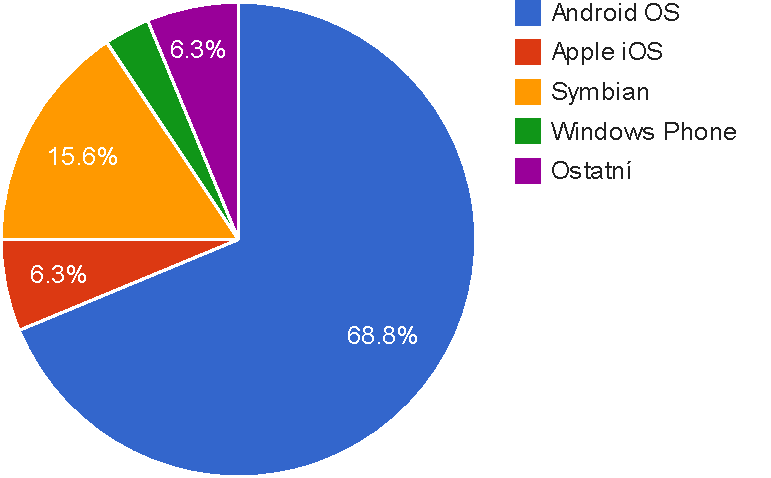
\includegraphics[scale=0.8]{charts/survey_os}
  \caption{Rozšíření mobilních platforem}
  \label{fig:SurveyOS}
\end{figure}

Výběr cílové platformy je tedy jistý. Čtenář může jistě dohledat další průzkumy rozšíření platforem, které jsou více či méně rozdílné. Všechny však poukazují na fakt, že OS Android je nejrozšířenější. Tato práce si klade za cíl poskytnout řešení pro tuto platformu. Protože budoucnost této aplikace může přinést rozšíření i na více platforem, je nutné zajistit, aby společné úložiště dat aplikace bylo možné použít i pro jinou platformu. Toto zajistí multiplatformní protokol.

Vzhledem k~tomu, že většina potravin disponuje čárovým kódem a k~tomuto kódu můžou být dohledány informace o~zboží, které identifikuje, lze aplikaci vybavit čtečkou čárových kódu, která usnadní manuální zadávání názvu či tohoto kódu pro identifikaci. Aby tato informace nebyla jen tak nadhozena, byla do dotazníku přidána další sekce. Na obrázku~\ref{fig:SurveyScan} lze pozorovat poměr mezi dotázanými, kteří by využili možnosti zadávat jídlo pomocí čtečky a těmi, kteří by toho nevyužili.

\begin{figure}[H]
  \centering
  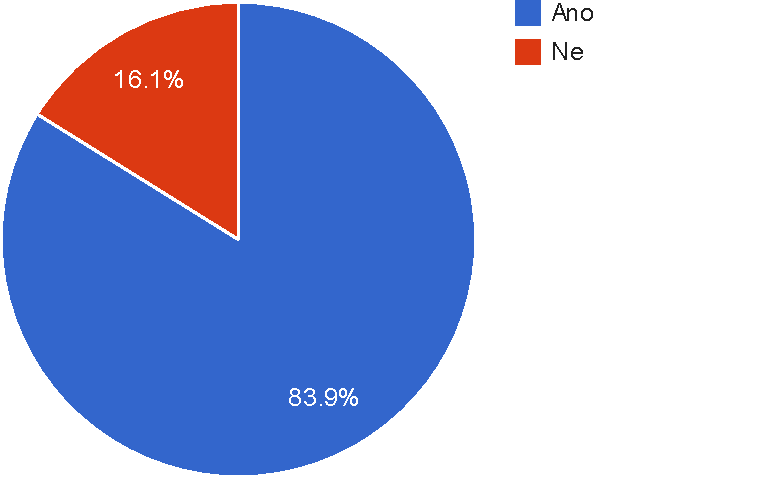
\includegraphics[scale=0.8]{charts/survey_scan}
  \caption{Žádanost zadávání potravin pomocí čtečky čárového kódu}
  \label{fig:SurveyScan}
\end{figure}

\section{Funkční požadavky}

Funkční požadavky této aplikace, které plynou z~daného problému a výše uvedených výsledků dotazníku jsou:
\begin{itemize}
  \item přidávání nových potravin
  \item sdílení známých potravin
  \item specifikace běžné doby spotřeby potravin
  \item zaznamenání obrázků potravin
  \item zaznamenávání potravin do inventáře
  \item odebírání potravin z~inventáře
  \item zaznamenání data spotřeby
  \item hledání potraviny pomocí čárového kódu nebo názvu
  \item čtení čárového kódu pomocí kamery mobilního telefonu
  \item čtení různě dlouhých čárových kódů
  \item upozornění na jídlo, jehož spotřební doba se již ocitla v~určitém intervalu blíže ke konci, či jehož spotřební doba již uplynula.
  \item nastavení intervalu pro upozornění o ukončení trvanlivosti, který je rozdílem data spotřeby potraviny a aktuálního data
  \item získávání informací o~neznámých potravinách z~otevřené databáze čárových kódů
\end{itemize}

OS Android se na cílových zařízeních nachází v~různých verzích. Některé jsou příliš staré na to, aby je bylo nutné podporovat, jiné jsou naopak ještě stále rozšířené. Pro přehled o~rošířených verzích lze shlédnout Android Dashboards ~\cite{dashboards}. Jak lze na diagramu vidět, od verze Android 2.3.3 a výše je rozšíření jednotlivých verzí významné, tedy má smysl tyto verze podporovat. To však s~sebou přináší některé odlišnosti a je třeba brát v~úvahu, že některé prvky API na nich nejsou k~dispozici. Tento fakt se snaží vyřešit Support knihovny~\cite{support}, které do starších verzí částečně přinášejí vlastnosti novějších API. V~průběhu implementace se bude dbát na průběžné testování na starších verzích, aby bylo dosaženo co nejlepší podpory starších verzí OS Android.

Čárové kódy na obalech potravin bývají různého formátu. Obecně se na nich objevují kódy typu GTIN. Kódy jsou číselné a mohou nabývat délky od 8 do 14ti číslic podle variant, které mají v názvu tento počet přímo zaznamenaný. Spolu se staršími názvy je jednotlivě vypíšu v následující tabulce\ref{table:carkod}.
\begin{table}[h]
      \begin{tabular}{|l|l|l|}
      \hline
      Název   & Počet číslic & Alternativní (starší) názvy \\ \hline
      GTIN-14 & 14           & DUN-14, ITF                 \\ \hline
      GTIN-13 & 13           & EAN·UCC-13, EAN-13, CIP     \\ \hline
      GTIN-12 & 12           & EAN·UCC-12, UCC-12, UPC     \\ \hline
      GTIN-8  & 8            & EAN·UCC-8, EAN-8            \\ \hline
      \end{tabular}
      \caption{Varianty čárových kódů typu GTIN}
      \label{table:carkod}
\end{table}
Kratší kódy lze snadno převést na delší doplněním nul do celkového počtu číslic, který je cílem převodu. Aplikace tedy vyžaduje možnost zaznamenání takových kódu.

\subsection{Čtečka čárových kódu}

Požadavek na čtení čárového kódu vyžaduje použití knihovny, která takovouto funckionalitu zvládne co nejlépe. Protože si práce klade za cíl využívat open-source software, nabízí se 2 známé otevřené knihovny. Předmětem této sekce bude popsat dostupné informace, zanalyzovat jejich praktické využití v~této aplikaci a vytvoření jednoduchého prototypu, který bude simulovat integraci do hotové aplikace.

Tuto sekci jsem zahrnul do analýzy, neboť přímo nepopisuje návrh, ale přináši analýzu knihoven, kterou pak lze dále použít v~návrhu a implementaci.

\subsubsection{Externí aplikace}

Čtečka čárových kódu by mohla být implementována pouze s pomocí externí aplikace. Zde však tento způsob naráží v~možnostech rychlosti zadávání čárového kódu. Pro spuštění externí aplikace je vyžadováno, aby se neustále přepínalo mezi jednotlivýmí aplikacemi, které vyústí v~pravidelném vypínání a zapínání snímacího čipu obrazu, čímž může dojít ke zpomalení. Samotné vyvolání externí aplikace trvá určitou dobu, takže celkové zpomalení bude určitě znatelné. Pro potvrzení tohoto tvrzení jsem vyzkoušel na dostupných zařízeních smyčku, která neustále zapínala a vypínala snímací čip. V~průměru bylo dosaženo na všech zařízeních času, který se pohyboval od 0,5 do 1 sekundy. Při vyvolávání externí aplikace bylo naměřeno v~průměru okolo 0,4 sekundy, protože je však nutné externí aktivitu opustit, tento čas je třeba ještě vynásobit dvěma. Ve výsledku tedy zpomalení dosahuje až 2 sekund. Pocitově takovéto zpomalení UI působí nepříjemně tím, že veškeré činnosti UI v~rámci aplikace po akci uživatele by měli být dokončené nejpozději do 1 sekundy ~\cite{ui_maxlag}. Delší časové prodlevy by vyžadovali nějaký prvek ukazující postup, který v~tomto případě spouštění externí aplikace není možný.

\subsubsection{Zbar ~\cite{zbar}}

Tato knihovna je šířena pod licencí GNU LGPL 2.1. Jazykem, ve kterém je knihovna implementována, je C. Díky tomu lze knihovnu snadno importovat na jakoukoliv platformu, která umožňuje spuštění nativního kódu. Android je takovouto platformou. Jeho NDK umožňuje zkompilovat a přiložit knihovnu k~aplikaci, ke které lze přistoupit pomocí rozhraní Javy, klíčovým slovem ``native''. Tímto NDK lze vygenerovat kód pro různé architektury, jako například ARM, MIPS, x86 a další varianty těchto předcházejících. Nevýhodou této knihovny je však fakt, že poslední vydaná verze byla v~roce 2010. Kód není dále aktivně vyvíjen.

Při vyzkoušení jednoduché ukázky knihovny vyšlo najevo, že nabízí nižší úspěšnost načítání čárových kódů oproti níže uvedené knihovně ZXing. Je tedy nutné zvážit fakt, zda-li je tato knihovna vhodná pro implementaci. Nenáročnost této knihovny mi však nepřipadá jako rozhodující faktor. Je to dáno především tím, že výkon zařízení neustále roste a tato výhoda přestává mít svoji váhu.

\subsubsection{ZXing ~\cite{zxing}}

Od autorů teamu ZXing (``Zebra Crossing'') této knihovny je na Play Store k~dispozici aplikace Barcode Scanner~\cite{barcode_scanner} využívající tuto knihovnu pro skenování širokého množství čárových i jiných vizuálních kódů. Tato knihovna je šířena pod licencí Apache License Version 2.0 a oproti knihovně Zbar je napsána v~jazyce Java. Touto cestou je knihovna snadno přenositelná do všech platforem podporujících Java byte kód nebo jiné, do kterých lze byte kód Javy převést. Tím je například Dalvik Virtual Machine používající Android.

Aplikace má sice vetší nároky na výkon zařízení, je však schopná číst velmi mnoho kódů, jejichž deaktivací se výkon dekódování obrazu ještě zvýší. Aplikace Barcode Scanner velmi dobře poslouží jako užitečný zdroj informací o~implementaci knihovny do vlastní aplikace. Aby byla aplikace co nejvíce užitečná, umožnuje s~výsledky provádět spoustu činností, jako vyhledávat kód v~různých databázích a rovnou zobrazovat výsledky bez externí aplikace. Kód této aplikace je tímto velice rozsáhlý a pro účely aplikace této práce je zbytečný, podle mě nepřehledný a tím pádem i špatně udržovatelný. Kódy GTIN jsou pouze malou podmnožinou všech, které tato aplikace spolu s~knihovnou podporuje, takže použití bude velice úzké, čímž jsem došel k~závěru, že bude vhodné implementovat vlastnosti aplikace a knihovny pouze do úrovně, která je nezbytná pro účely této práce.

Velikou výhodou této knihovny je především aktivní vývoj, lze tudíž do budoucna počítat se spolehlivějším načítáním kódu i vyšší efektivitou knihovny. Veškeré zdrojové kódy knihovny ZXing a její implementující aplikace Barcode Scanner jsou k~dispozici pod stejnou licencí. Je tedy možné využít jakoukoliv část těchto kódu i v~rámci této práce. 

\subsubsection{Implementace prototypu}

Pro implementaci prototypu autor zvolil knihovnu ZXing a vhodné části aplikace Barcode Scanner zejména proto, aby se seznmámil s~její strukturou a vniřními mechanismy. 

\subsubsection{Výsledek implementace}

Vytvořen byl prototyp obsahující pohled kamery, status panelem a jednoduchým formulářem. Snímek obrazovky prototypu na zařízení Nexus 7 si lze prohlídnout na obrázku~\ref{fig:ScanPrototype}. Implementace využívá části kódu původní aplikace Barcode Scanner, hlavní změnou však je použití vyššího rozlišení a jiný způsob prezentace výsledků. Původní komunikace mezi komponentami zůstala stejná, mnoho tříd však bylo odděděno z~důvodu nutnosti upravit mnoho detailů, které způsobila provázanost veškerých tříd na sobě, čímž byla způsobena velice špatná upravitelnost a udržovatelnost kódu. Na základě prototypu se autor této práce rozhodl ve finální aplikaci nepoužívat žádný kód původní aplikace Barcode Scanner ani tohoto prototypu a vyvinout vlastní skenovací komponenty s~pomocí samotné knihovny ZXing, které budou mnohem jednodušší a tím pádem i snadněji udržovatelné a přizpůsobitelné.

Změna na vyšší rozlišení se z~používaní prototypu pro skenování různých potravin ukázala jako vhodná na všech zmíněných zařízeních. Zařízení Vodafone 845 však nemá možnost zaostřit na blízký předmět a jelikož disponuje pouze nízkým rozlišením, tak výsledků, které by změna zlepšila, mnoho nebylo. Použitelné se ukázali pouze veliké čárové kódy snímané z~větší vzdalenosti, aby se dosáhlo optimálního ohniska čočky ostřící obraz. Odproštění od ostatních formátů kódů z původní aplikace Barcode Scanner však znamenalo pocitově velmi znatelný pokles snímací doby, kterou způsobila detekce všech podporovaných čárových kódů. Zvýšení rozlišení obrazu dále nepatrně snímací dobu prodloužilo, ale aplikace je takto schopná detekce čárového kódu ve větším rozsahu vzdálenosti.

\begin{figure}[H]
  \centering
  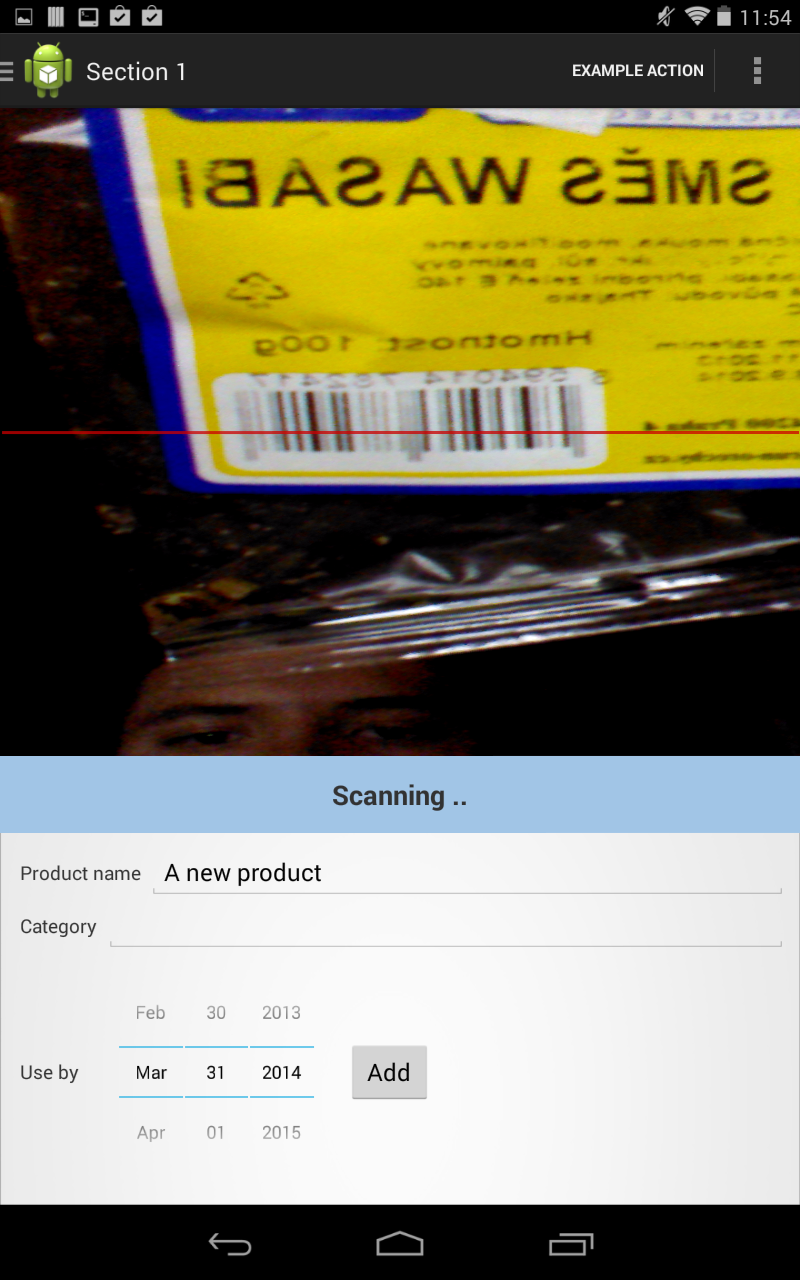
\includegraphics[scale=0.3]{screenshots/scan_prototype.png}
  \caption{Prototyp snímaní čárových kódů}
  \label{fig:ScanPrototype}
\end{figure}

\section{Nefunkční požadavky}

Externí úložiště aplikace bude tvořit server. Plánuji nasazení serveru na stroj, který nedisponuje příliš vysokým výkonem ani velikostí operační paměti. Z~tohoto důvodu je kladen na server požadavek na nízkou paměťovou stopu a efektivitu implementace, která nezatíží serverový stroj. Dále však plánuji do budoucna server nasadit na výkonější stroj. Je tedy důležité zajistit, aby server dokázal lepších parametrů serveru využít.

Server budé dále umožňovat připojení z~více zařízení v~rámci jednoho uživatele se stejným účtem, aby zajistil používaní například v~rámci rodiny. 

Pro celou práci se snažím využívat zdarma dostupných nástrojů a využít již hotového software, který je dodáván pod open-source licencemi. Samotný kód aplikace hodlám publikovat jako open-source software, aby následně po skončení práce mohl být vylepšován i případnými zájemci.

Seznam nefunkčních požadavků:

\begin{itemize}
  \item platforma OS Android
  \item rychlost zadávání potravin do inventáře
  \item multiplatformní protokol pro mobilní aplikaci a externí úložiště dat
  \item nenáročnost serveru
  \item výkonová škálovatelnost serveru
  \item dostupnost serveru z~více zařízení jedním účtem uživatele
  \item využití open-source software
\end{itemize}


\chapter{Návrh}

Kapitola návrh poskytne soubor informací k~následné implementaci. Požadavky sepsány v~kapitole analýzy budou diktovat jeho obsah. Struktura návrhu se týka popisu případů užití, návrhu architektury, doménového modelu, databázového modelu a popisu komunikačního protokolu.

\section{Případy užití}

Výše uvedené funkční požadavky se přimo promítají do případů užití. Tento diagram slouží pří návrhu UI i pro tvorbu scénářů pro usability testing, které ověří, zda daný návrh je pro uživatele dostatečne jednoduchý a zda-li je uživatel schopen v~aplikaci dosáhnout všech daných cílů.

Inventář a vyhledání potraviny jsou základnami, ze kterých se dále odvíjejí ostatní činnosti. Jednotlivé případy vystihují přesně ty činnosti, které bude uživatel provádět během používání aplikace.

Při vytváření tohoto diagramu byl dán veliký důraz na nejčastější činnosti uživatele, které lze očekávat. V~závěru práce dojde ke zhodnocení zde navrhnutých scénářů a přípádné návrhy na změnu do budoucnosti.

\begin{figure}[H]
  \centering
  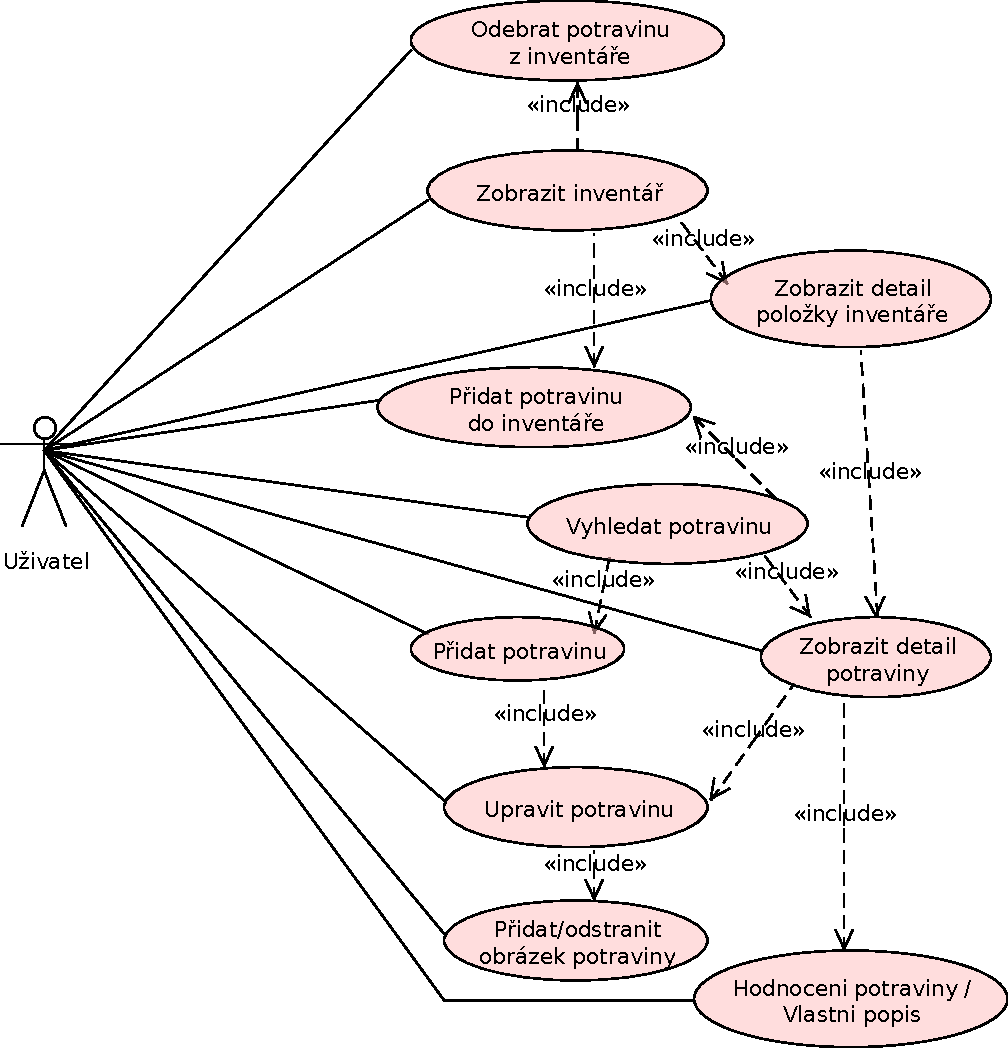
\includegraphics[scale=0.75]{diagrams/use_case}
  \caption{Diagram případů užití}
  \label{fig:UseCase}
\end{figure}

\section{Architektura}

Vzhledem k nutnosti použít pro mobilní aplikaci server bude nejvhodnější model architektury klient - server. Tento model vyžaduje specifikovat komunikaci mezi oběma stranami a dále při vhodném navrhnutí lze uvažovat i o~klientech pro více platforem. Vhodná platforma pro jiný typ aplikace by mohla být webová aplikace, která by zpřístupňovala aplikaci na všech ostatních platformách skrze webový prohlížeč. Touto cestou by však nebylo možné uživatele jednoduše upozorňovat o~trvanlivosti přímo z~webové stránky i v~době, kdy uživatel stránku neprohlíží.

\subsection{Klient}

Z~nefunkčního požadavku OS Android vyplývá nutnost implementovat aplikaci s~pomocí jeho SDK. Existují multiplatformní SDK nabízející bežné API, avšak nutnost vytváření upozornění a snímaní čárových kódů je čistě specifická záležitost pro kažou platformu zvlášť. Tuto možnost autor předpokládá jako časově náročnou, proto se tato práce soustředí pouze na Android SDK.

\subsection{Server}

Jako jeden z~hlavních požadavků na server je jeho malý paměťový otisk. Nabízí se spousta různých variant, jak tohoto cíle dosáhnout. Jelikož předměty prvního ročníku mého studia obsahovali především algoritmizace v~jazycích C/C++ a obor softwarového inženýrství si vyžádal předmět efektivních algoritmů, byla jako vhodná varianta serveru jeho implementace v~jazyce C++. Bližší detaily jeho návrhu budou priblíženy dále.

\section{Doménový model}

Na obrázku doménového modelu ~\ref{fig:DomainModel} lze spatřit vztahy mezi všemi entitami, jejichž význam zde bude vysvětlen.

\subsection{Category}
Category poskytuje kategorizaci potravin. Tato entita je připravena pro budoucí rozšíření vyhledávání, v~rámci této práce je informace o~kategorii pouze shromažďována jako název.

\subsection{Edit}
Každá editace potraviny tvoří záznam entity Edit, ve které se nachází informace kdo, kdy a co upravil. Tato informace poté může sloužit k~blokování škodlivých uživatelů a k nahrazení dat, které tyto uživatelé poškodili.

\subsection{Food}
Entita food popisuje potravinu jako název, výchozí trvanlivost, běžnou cenu, kategorii, výrobce a uživatele, který potravinu do aplikace přidal.

\subsection{Image}
Každá potravina může nabýt předem nespecifikovaného množství obrázků od uživatelů. Zde je zaznamenán pouze uživatel, který obrázek k potravině přidal.

\subsection{Inventory}
Položka inventáře spojuje uživatele a potravinu, která zároveň určuje datum spotřeby. Při přidání několika instancí potraviny do inventáře najednou se vždy přidá stejný počet záznamů této entity.

\subsection{Review}
Jednoduché hodnocení potraviny od 0 do 5 s~volitelným textem recenze uživatele. Každý uživatel může nabýt nejvíce jednoho hodnocení.

\subsection{User}
Entita uživatele uchovává pouze uživatelské jméno. Tuto entitu bude nutné v~budoucnu rozšířit o~příslušné vlastnosti v~případě, že bude třeba uživatelská data více zabezpečit.

\subsection{Vendor}
Výrobce je specifikován jako samostatná entita, v~budoucnu lze také použít pro filtrování vyhledávání stejně jako je tomu u~kategorie.

\begin{figure}[H]
  \centering
  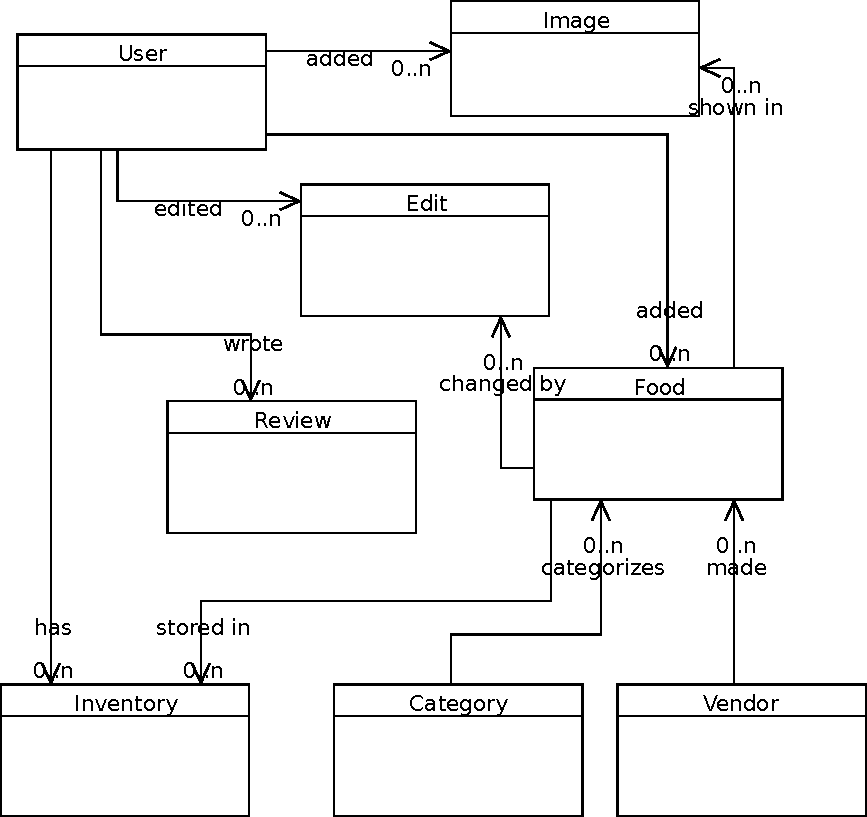
\includegraphics[scale=0.75]{diagrams/model}
  \caption{Doménový model}
  \label{fig:DomainModel}
\end{figure}

\section{Databázový model}

Z~protředků cílového stroje určeného k~nasazení serveru této aplikace byl jako databázový software zvolen MySQL. K~návrhu jsem využil software MySQL Workbench, který umožnuje vytvořit relační model, který je přímo kompatibilní s~vlastnostmi MySQL. Jelikož jsou veškerá data aplikace uchovávána na serveru, vychází relační model přímo z~doménového. Entity tedy zůstávají stejné.

Některé atributy entit nemusí být zcela jasné, proto jsem níže vypsal entity s vybranými atributy do sekcí, kde se je pokouším čtenáři přiblížit.

\subsection{Edit}

Atribut \textbf{message} zaznamenává zprávu editace. V té server ukládá informaci o tom, jaká editace byla provedena. Případně se tam mohou objevit další zajímavé informace, které poslouží při správě dat o potravinách, tedy k blokování uživatelů, jak již bylo výše zmíněno.

\subsection{Food}

\textbf{gtin} zaznamenává kód GTIN v mém vlastním formátu, který tvoří dohromady 15 znaků. První znak označuje typ čárového kódu v pořadí. Tyto znaky mohou být A, B, C, D nebo Z, které přímo odlišují ve stejném pořadí délky GTIN kódů 8, 12, 13 nebo 14 znaků. Zbylých 14 znaků je vždy samotný kód GTIN doplněný o počáteční nuly do celkové délky.

\textbf{default\_use\_by} zaznamenává dobu běžné spotřeby v unixovém času v milisekundách. Tento typ formátu jsem zvolil pro jednoduchost uložení časového období a následného počítaní s ním.

\textbf{amount\_measure} pro atribut \textbf{amount}, který zaznamenává nějaké množství, popisuje jakým typem množství tato potravina disponuje. Níže je seznam popisující jednotlivé typy.

\begin{itemize}
  \item 0 s názvem konstanty AMOUNT\_TYPE\_GRAMS popisuje množství v počtu gramů
  \item 1 s názvem konstanty AMOUNT\_TYPE\_LITRES popisuje množství v počtu litrů
  \item 2 s názvem konstanty AMOUNT\_TYPE\_PIECES popisuje množství v počtu kusů
\end{itemize}

\textbf{price} ukládá běžnou cenu potraviny jako hodnotu v americkém dolaru.

\subsection{Inventory}
V atributu \textbf{use\_by} je uložen datum, do kterého by se měla daná potravina s klíčem v atributu \textbf{food\_id} spotřebovat.

\subsection{Review}
\textbf{rating} atribut zaznamenává reálnou hodnotu hodnocení potraviny \textbf{food\_id} v rozsahu 0 až 5.


\begin{figure}[H]
  \centering
  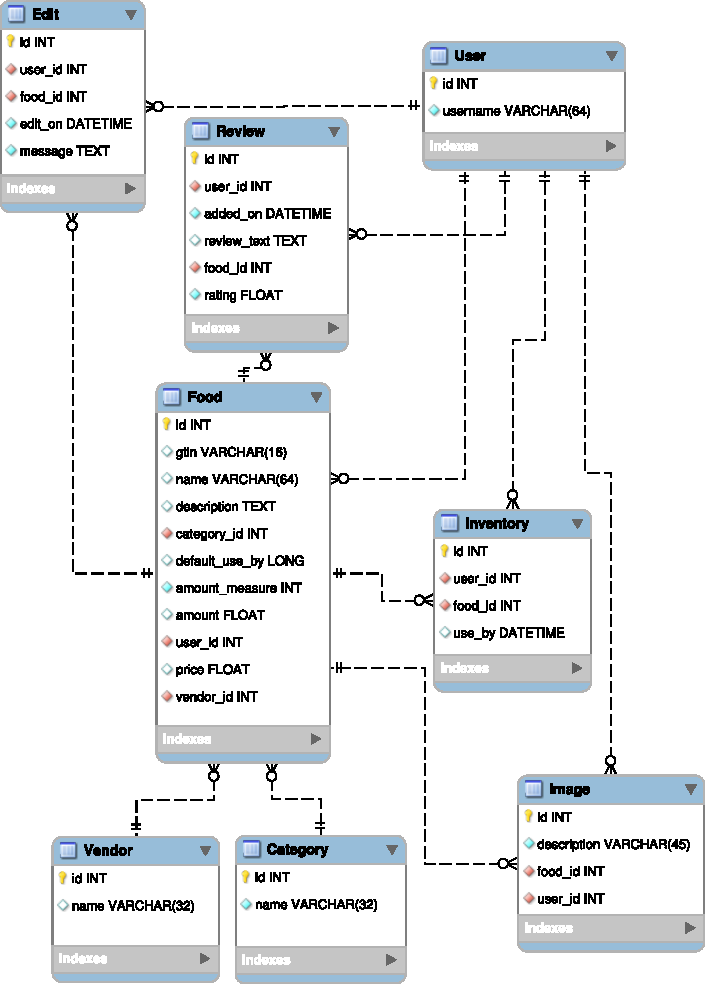
\includegraphics[scale=1.20]{diagrams/relational_model}
  \caption{Relační model}
  \label{fig:RelationalModel}
\end{figure}


\section{Komunikační formát a protokol}

Z~důvodu zvolené architektury je nutné specifikovat protokol, jakým budou mezi sebou komunikovat klient a server. Android SDK diktuje pro mobilního klienta použití jazyku Java, který sice lze nahradit pomocí C/C++, toho se však doporučuje jen v~aplikacích či knihovnách s~potřebou vysokého výkonu nebo přístupu k~hardware ~\cite{android_ndk}. Tato odlišnost vyžaduje použít platformě nezávislý protokol na bázi například textu.

\subsection{XML}

Mnoho protokolů využíva ke komunikaci textový formát v~XML. Tento formát je podobný HTML, je platformově nezávislý a široce podporován. V~C/C++ ho implementují různé knihovny, které jsou dostupné jako open-source software. Formát však nevyžívá datový prostor dostatečně efektivně, jak bude popsáno dále.

\subsection{JSON}

Jako další textový formát umožňující platformově nezávislý přenos dat je JSON. Je to velice populární formát používaný široce ve webových technologiích a jeho použití je také velmi jednoduché. Formát vychází z~JavaScriptové notace a lze ho s~bezpečnostními opatřeními proti vložení zákeřného kódu načíst jako samotný zdrojový kód JavaScriptu. Výhodou formátu JSON je jeho kompaktnost oproti formátu XML, čímž dojde ke snížení přenášeného množství dat a přesto se zachová textový formát reprezentace dat.

\subsection{Porovnání a zvolení formátu}

Oba formáty jsou přímo podporovány v~Android API a tak jsou vhodnými kandidáty. Od obou formátů jsou k~dispozici různé kompaktnější verze, které ještě více data zhušťují nebo využívají jiné kompresní algoritmy pro snížení velikosti jejich dat. Využití takovýchto vylepšení je však omezující jeho podporou různých prostředí a neumožňují lidsky čitelný formát, který je vhodný pro vývoj a odhalování chyb.

Různé knihovny implementují tyto formáty i do C++, které jejich podporu ve standardních knihovnách neobsahuje. Jelikož jediný patrný rozdíl je ve větší kompaktnosti, byl zvolen JSON jako formát protokolu pro tuto aplikaci.

\subsection{Struktura protokolu}

Protokol budou tvořit zprávy, které budou mít pevný tvar. Kvůli možnosti budoucího vylepšení protokolu například do komprimované podoby a jednoduchosti jeho načtení ze síťového proudu je vhodné poslat přesný počet bytů každé zprávy v~pevně daném pořadí. Zpráva bude mít teoreticky neomezenou velikost, avšak server bude mít možnost tuto velikost omezit kvůli zabránění zahlcení serveru jednoduchým útokem, který by zaplnil celou dostupnou pamět a způsobil pád serveru. Maximální velikost zprávy bude možné nastavit v~serveru a bude to také hodnota, která s~dalšími vlastnostmi určí maximální množství uživatelů, který je server schopen v~extrémním případě obsloužit.

Komunikaci budou tvořit zprávy přenesené v~přesném pořadí jako:

\begin{itemize}
  \item{4 byty určující celé číslo N v~Big Endian pořadí, stejné jako Network Byte Order}
  \item{N bytů textové UTF-8 zprávy}
\end{itemize}

Zprávy budou mít dále již v~JSON formátu strukturu:
\begin{lstlisting}
{
  "header" : "NazevZpravy",
  "content" :
    {
      .. dalsi obsah zpravy ..
    }
}
\end{lstlisting}

\begin{itemize}
  \item{položka header určuje název zprávy, který bude popsán dále}
  \item{položka content obsahuje položky určité zprávy}
\end{itemize}

Zprávy budou mít povahu požadavku a odpovědi na něj. Klient bude posílat serveru požadavky a ten mu na ně příslušně odpovídat. Neznámé zprávy způsobí ukončení komunikace.

Jednotlivé zprávy byly navrženy již s~ohledem na funkce uživatelského rozhraní. Tyto zprávy budou dále popsány. Zprávy kromě poslední KeepAlive jsou dvojice Request a Respond, např. pro zprávu Login to je LoginRequest a LoginResponse.

\subsubsection{Login}
Přihlásí uživatele pod jménem (e-mailem) a vrátí odpověď jako boolean, true pro úspěch a false při selhání přihlášení.

Položky požadavku:
\begin{itemize}
  \item \textbf{username} - email jako jméno uživatele
\end{itemize}

Položky odpovědi:
\begin{itemize}
  \item \textbf{success} - boolean, true pokud úspěšné přihlášení
  \item \textbf{message} - v případě neúspěchu přihlášení je zde popsán důvod
\end{itemize}

\subsubsection{GetInventory}
Vyhledá a vrátí množinu položek inventáře podle zadaného jména, kódu GTIN nebo přímo pomocí unikátního id.

Položky požadavku:
\begin{itemize}
  \item \textbf{direct} - boolean, hodnota určuje, zda-li je požadavek mířen přímo na id položky inventáře nebo je hledána množina podle dalších atributů
  \item \textbf{id} - unikátní identifikátor položky inventáře
  \item \textbf{food} - název potraviny, která je hledána, nebo jen jeho část
  \item \textbf{gtin} - číslo GTIN potraviny, která je hledána, nebo jen jeho část
\end{itemize}

Položky odpovědi jsou uloženy v atributu \textbf{items}, disponují následujícími atributy:
\begin{itemize}
  \item \textbf{id} - unikátní identifikátor položky inventáře
  \item \textbf{foodId} - unikátní identifikátor potraviny
  \item \textbf{imageId} - unikátní identifikátor nějakého obrázku, pokud existuje, jinak 0
  \item \textbf{foodName} - název potraviny
  \item \textbf{foodGtin} - číslo GTIN
  \item \textbf{useBy} - unixový čas dne v milisekundách (od roku 1970), kdy končí trvanlivost potraviny
\end{itemize}

\subsubsection{GetFoodDetail}
Vratí veškeré detaily potraviny.

Položky požadavku:
\begin{itemize}
  \item \textbf{id} - unikátní identifikátor potraviny
\end{itemize}

Položky odpovědi jsou uloženy v atributu \textbf{items}, disponují následujícími atributy:
\begin{itemize}
  \item \textbf{id} - unikátní identifikátor potraviny
  \item \textbf{name} - název potraviny
  \item \textbf{category} - název kategorie
  \item \textbf{categoryId} - unikátní identifikátor kategorie
  \item \textbf{vendor} - název výrobce potraviny
  \item \textbf{vendorId} - unikátní identifikátor výrobce potraviny
  \item \textbf{gtin} - čislo GTIN
  \item \textbf{imageIds} - pole unikátní identifikátorů obrázků
  \item \textbf{description} - popis potraviny
  \item \textbf{defaultUseBy} - výchozí datum spotřeby
  \item \textbf{amountType} - množstevní typ potraviny
  \item \textbf{amount} - množství potraviny
  \item \textbf{usualPrice} - obvyklá cena v amerických dolarech
  \item \textbf{reviews} - položky jednotlivých hodnocení uživatelů
  \item \textbf{addedBy} - jméno uživatele, který potravinu přidal
  \item \textbf{lastEditedBy} - jméno uživatele, který potravinu poslední upravil
\end{itemize}

\subsubsection{GetFoodItem}
Vyhledá a vrátí množinu potravin podle jména nebo GTIN kódu.

Položky požadavku:
\begin{itemize}
  \item \textbf{direct} - boolean, hodnota určuje, zda-li je požadavek mířen přímo na id potraviny nebo je hledána množina podle dalších atributů
  \item \textbf{id} - unikátní identifikátor potraviny
  \item \textbf{food} - název potraviny, která je hledána
  \item \textbf{gtin} - číslo GTIN potraviny, která je hledána
  \item \textbf{skip} - počet položek, které se mají při výberu přeskočit
\end{itemize}

Položky odpovědi jsou uloženy v atributu \textbf{items}, disponují následujícími atributy:
\begin{itemize}
  \item \textbf{id} - unikátní identifikátor potraviny
  \item \textbf{defaultUseBy} - výchozí datum spotřeby
  \item \textbf{imageId} - unikátní identifikátor nějakého obrázku, pokud existuje, jinak 0
  \item \textbf{name} - jméno potraviny, která je hledána, nebo jen jeho část
  \item \textbf{desc} - popis potraviny
  \item \textbf{gtin} - číslo GTIN potraviny nebo jen jeho část, které je hledáno
\end{itemize}


\subsubsection{EditInventory}
Upraví položku inventáře.

Položky požadavku:
\begin{itemize}
  \item \textbf{adding} - boolean, true pokud položka inventáře ještě neexistuje a je vytvářena
  \item \textbf{id} - unikátní identifikátor položky inventáře
  \item \textbf{foodId} - unikátní identifikátor potraviny
  \item \textbf{useBy} - datum spotřeby v unixovém čase v milisekundách
  \item \textbf{count} - počet položek inventáře, které se mají vytvořit se stejnými parametry
\end{itemize}

Položky odpovědi:
\begin{itemize}
  \item \textbf{success} - boolean, true pokud editace položky inventáře dopadla v pořádku
\end{itemize}

\subsubsection{DeleteInventory}
Smaže položku inventáře.

Položky požadavku:
\begin{itemize}
  \item \textbf{id} - unikátní identifikátor položky inventáře
\end{itemize}

Položky odpovědi:
\begin{itemize}
  \item \textbf{success} - boolean, true pokud úspěšné smazáno
\end{itemize}

\subsubsection{EditFood}
Upraví detail potraviny.

Položky požadavku jsou shodné s detailem potraviny a analogicky stejná s editací položky inventáře. Neobshají však pole identifikátorů obrazků a hodnocení uživatelů.

Položky odpovědi:
\begin{itemize}
  \item \textbf{success} - boolean, true pokud úspěšná editace potraviny
  \item \textbf{id} - unikátní identifikátor přávě vytvořené potraviny
\end{itemize}

\subsubsection{GetFoodBase}
Vrátí výrobce a kategorie k~zadání potraviny.

Požadavek nemá žádné položky.

Položky odpovědi:
\begin{itemize}
  \item \textbf{vendors} - pole všech známých výrobců
  \item \textbf{categories} - pole všech známých kategorií
\end{itemize}

\subsubsection{AddImage}
Nahraje nový obrázek potraviny.

Položky požadavku:
\begin{itemize}
  \item \textbf{imageData} - řetězec s daty obrázku při základu 64 zakódované jako textové znaky, který zabírá zhruba o 0,334 krát větší místo než původní binární reprezentace, což jsem uznal za uspokojující
  \item \textbf{foodId} - unikátní identifikátor potraviny
\end{itemize}

Položky odpovědi:
\begin{itemize}
  \item \textbf{success} - boolean, true pokud úspěch
\end{itemize}

\subsubsection{DeleteImage}
Smaže zadaný obrázek potraviny.

Položky požadavku:
\begin{itemize}
  \item \textbf{id} - unikátní identifikátor obrázku
\end{itemize}

Položky odpovědi:
\begin{itemize}
  \item \textbf{success} - boolean, true pokud úspěšné smazání obrázku
\end{itemize}

\subsubsection{SetUserReview}
Vytvoři, nastaví nebo smaže uživatelovu recenzi.

Položky požadavku:
\begin{itemize}
  \item \textbf{rating} - hodnocení potraviny v reálném čísle
  \item \textbf{delete} - boolean, true pokud se má recenze pro aktuálního uživatele odstranit, jinak vytvořit či změnit
  \item \textbf{foodId} - unikátní identifikátor potraviny
  \item \textbf{text} - text hodnocení uživatele
\end{itemize}

Položky odpovědi:
\begin{itemize}
  \item \textbf{success} - boolean, true pokud úspěch požadavku
\end{itemize}

\subsubsection{KeepAlive}
Příkaz udržující spojení po dobu od posledního, neobsahuje žádné atributy.

\section{Server}

Z~výše uvedených požadavků lze vypsat tyto vlastnosti, které musí server splňovat:

\begin{itemize}
  \item{Implementace v~C++}
  \item{Škálovatelnost}
  \item{Zdroj dat z~MySQL}
  \item{Implementace protokolu s~JSON formátem}
\end{itemize}

Následující podsekce popisují zvolené detaily těchto vlasntostí.

\subsection{C++}

Implementace v~C++ se může zdát jako silně platformově závislá. Opak je však pravdou. Pro implementaci serveru jsem totiž zvolil ISO C++ standard C++11, který mimo jiné přináší multiplatformní podporu multithreading. Dále také umožňuje tvořit snadněji určité konstrukce, které byly dříve obtížnější. Díky těmto vlastnostem by následná implementace serveru měla být jednodušší, neboť není třeba příliš uvažovat o~rozdílech jednotlivých platforem až na vytváření serverového socketu, které je ale velice podobný na všech používaných platformách a jeho přizpůsobení je tím pádem velice jednoduché.

\subsection{Škálovatelnost}

Aby bylo možné server přizpůsobit výkonějšímu hardware, je třeba příslušné škálovatelnosti. V~případě této práce se jako její nejjednodušší forma jeví použití vlákna pro každého připojeného uživatele zvlášť. Je však také nutné zajistit, že další prostředky jako například připojení k~databázi bude pro vlákna dostupné soubežně a tím umožní zpracovávat více databázových dotazů současně. Je to důležite zejména proto, že tyto operace jsou obecně časově nejnáročnější. Tato forma škálovatelnosti však umožní získat vyšší výkon pouze za předpokladu, že dojde ke zvýšení počtu výpočetních jednotek, které mohou provádět instrukce jednotlivých vláken současně.

Jako další forma škálovatelnosti se již nabízí pouze přizpůsobení větší dostupné dynamické paměti. Zde jde třeba zdůraznit, že navrhnutý komunikační protokol vyžaduje určitou paměťovou režii kvůli dále zmíněné knihovně pro podporu JSON. Server tedy bude mít možnost upravit maximální počet současně obshluhovaných uživatelů, který bude závislý na dostupné paměti.

\subsection{MySQL}

Pro pohodlné a jednoduché použití MySQL v~C++ je vhodné využít rozhraní jiné než poskytované samotnou klientskou knihovnou, které není optimalizováno pro objektové použití v C++ a přináší tak s sebou mnohem složitější implementaci. Jako vhodná multiplatformní knihovna poskytující takové rozhaní se jeví MySQL Connector/C++~\cite{mysqlconn}. Tato knihovna nabízí rozhraní velmi podobné s~tím, co je dostupné pro použití v~jazyce Java. Lze tedy použít například PreparedStatement, které ošetří případné útoky pomocí pokoření formátu dotazů a podobné. Dále poskytuje vyjímky pro běžné chyby, které mohou nastat v~rámci jejího použití. Je tedy vhodná pro objektově návržený server. Kromě těchto vlastností umí také poskytovat více připojení k~samotnému databázovému serveru, takže poskytne vyžadovanou škálovatelnost z~podsekce výše.

\subsection{JSON}

Knihoven podpory JSON pro použití jazykem C++ je mnoho. Nejrozšířenější knihovny, které se mi podařilo nalézt jsou: rapidjson, JsonCpp, LibJSON. Knihovny jsou si velmi podobné, neboť specifikace formátu JSON není příliš rozsáhlá. Po delším prohlížení zdrojových kódů jednotlivých knihoven a jejich příkladů použití jsem si vybral knihovnu JsonCpp, která se mi jevila jako nejjednodušší a nejsrozumitelnější. Tato knihovna umožňuje použití prvků formátu JSON jako objekty a výrazně tak zjednodušuje jejich integraci do serverové aplikace. Knihovna je také multiplatformní.

Při testování zmíněné knihovny JsonCpp však vyšlo najevo, že knihovna nepoužívá vyjímky pro zachycení nejrůznejších chyb. Některé chyby způsobily přímo pád serverové aplikace. Tuto vlastnost tedy bylo třeba povolit. Tato úloha se však ukázala jako velmi jednoduchá.

Jelikož distribuovaná verze JsonCpp, která je bežně dostupná, vyjímky nevyhazuje, je třeba do serveru přidat počateční test, který ověří, zda-li je možné odchytit chyby při použití této knihovny. V případě, že tomu tak není, test následně upozorní uživatele, který se server pokouší spoustit.

Pro podporu vyjímek byl zřízen speciální repozitář~\cite{json_ex_repo} s~aplikovaným patchem pro tuto vlastnost. Použití této upravené verze je tedy nutnost pro bezchybný běh serveru.

\subsection{Návrh tříd}

Protože návrh tříd je příliš rozsáhlý, není vhodné ho zde prezentovat. Detailnější informace jsou dostupné v~rámci hlavičkových souborů v~poskytnutých zdrojových kódech k~této práci.

\section{Klient}

Jelikož klient této aplikace slouží jako rozhraní pro uživatele, je třeba dbát na návrh uživatelského rozhraní co nejvíce. Návrh klienta dále popisuje další klíčové oblasti, které je nutné správně navrhnout.

\subsection{Uživatelské rozhraní}

Při návrhu jsem dbal především na požadavek jednoduchosti. Tvorba uživatelského rozhraní je možná v~různém softwaru. V~případě OS Android je však návrh proveditelný přímo do spustitelné podoby s~pomocí vývojářských nástrojů. Tento postup s~sebou přínáší následující výhody:

\begin{itemize}
  \item{Jednoduchost návrhu - nástroje jsou velmi intuitivní}
  \item{Nástroje umožňují předem získat přehled o~vzhledu na různých typech a velikostech obrazovek}
  \item{Vytvořený návrh lze okamžitě testovat mezi dobrovolníky zasláním aplikace}
  \item{Výsledná podoba návrhu již nemusí být vytvářena znova a lze využít již hotový návrh pro finální aplikaci}
\end{itemize}

Pro běžný návrh UI jsou používány wireframy. Ty jsem však vynechal a místo toho jsem vyvíjel UI přímo pomocí vývojářských nástrojů, které mi umožnili získat přesnější podobu rozhraní a získat přehled o tom, jaké prvky UI lze využít pro dosažení cílů návrhu. Tím jsem však vývoj nijak nezpomalil, neboť z vlastní zkušenosti vím, že tvorba wireframů je přibližně stejne složitá jako rozmístění prvků UI v těchto nástrojích.

Dále je zobrazen UI diagram ~\ref{fig:UIDiagram}, ve kterém je možné spatřit jednotlivé názvy obrazovek a akce, pomocí kterých se uživatel mezi obrazovkami naviguje. Poté jsou ještě níže popsány vybrané obrazovky zajímavé pro uživatele.

\begin{figure}[H]
  \centering
  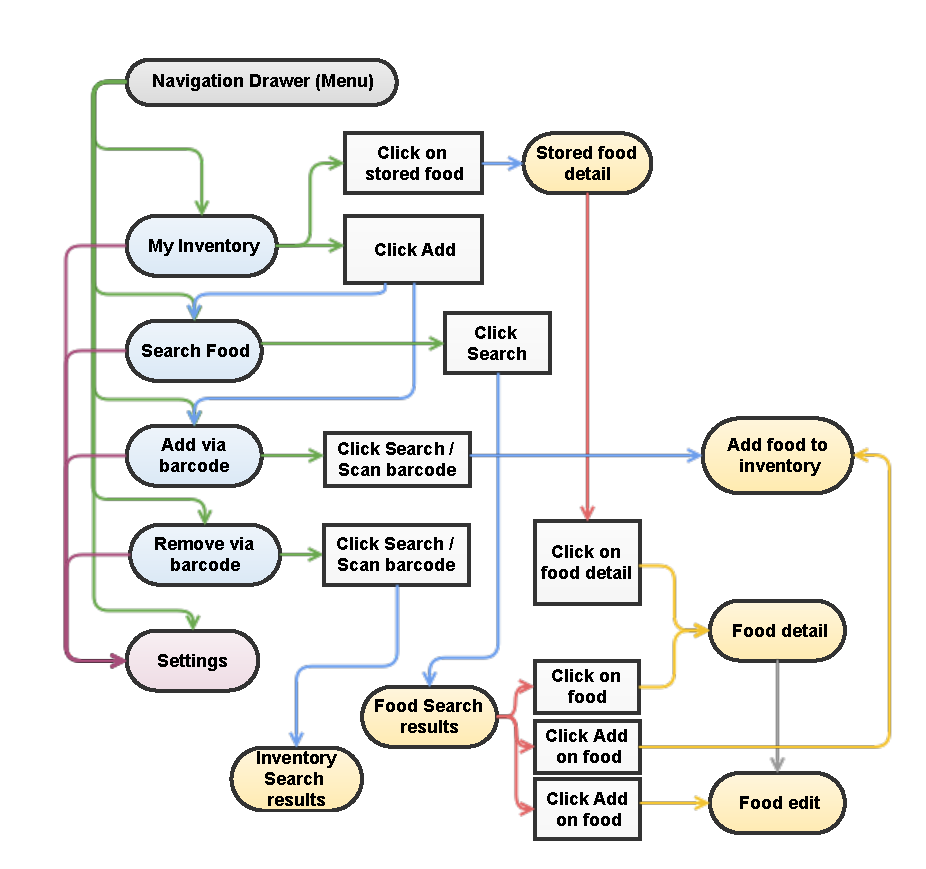
\includegraphics[scale=0.70]{diagrams/ui.pdf}
  \caption{UI Diagram s obrazovkami v zaoblených obdélnících a akcemi ve zbývajících. Zpětné šipky jsou pro přehlednost vynechány. Z obrazovek se však lze dostat ve směru při průchodu zleva doprava opačným směrem zpátky pomocí tlačítka zpět.}
  \label{fig:UIDiagram}
\end{figure}

\clearpage

\subsubsection{Menu}

První obrazovkou, kterou uživatel po spuštění aplikace uvidí, je navigační menu na obrázku~\ref{fig:AppMenu}. Je přímo dostupné ze všech cílu položek tohoto menu stiskem tlačítka v~horní levé části nebo posunutím ukazatele (prstu) od okraje obrazovky do jejího středu. Z~ostatních podpoložek se lze dostat zpět standardně tlačítkem zpět, případně tlačítkem v~horním panelu, tzv. ActionBaru.

Důvod existence pouze těchto položek spočívá v~jednoduchosti navigace. Scénář použití vždy začíná v~jedné z~těchto položek. Nastavení je dostupné standardně přes stisk klávesy menu nebo přes ikonu menu v~ActionBaru. Stejné je to s~nastavením i na ostatních obrazovkách.

\begin{figure}[H]
  \centering
  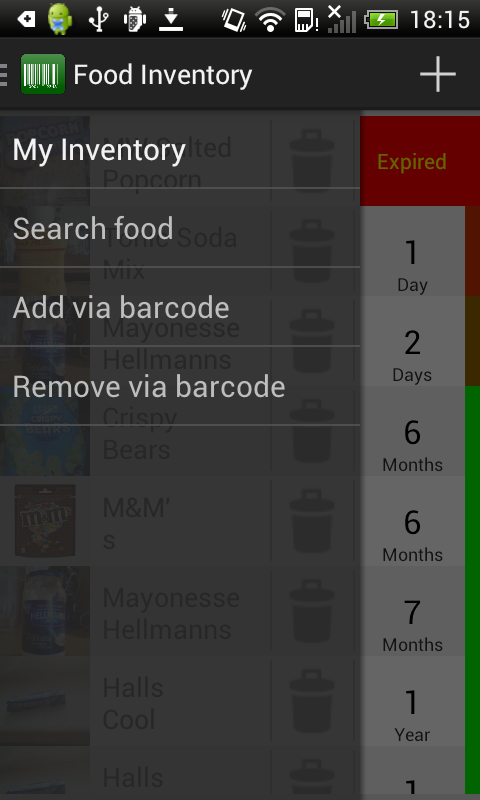
\includegraphics[scale=0.4]{screenshots/app_menu.png}
  \caption{Menu aplikace}
  \label{fig:AppMenu}
\end{figure}

\clearpage

\subsubsection{Inventář}

Inventář se stejně jako menu zobrazí při prvním spuštění, zůstane však v~jeho pozadí. Zachycuje ho obrazovka~\ref{fig:AppInventory}. Je zde možné pozorovat seznam potravin, které vlastní uživatel. Tyto položky inventáře dále disponují datumem spotřeby, díky kterému docházi k~seřazení a následně je u~potravin barevně vyznačen jejich status trvanlivosti. Červeně jsou vyznačeny potraviny s~končící trvanlivostí a postupně přechodem do zelené ty, které jsou od konce trvanlivosti vzdáleny více než týden.

Každá položka inventáře reaguje na stisk uživatelem. Při stisku dojde k~zobrazení detailu položky, který je popsán dále. Pro odebrání je k~dispozici ikona odpadkového koše, který potravinu z~inventáře odstraní.

Přidání nové položky do inventáře bude nejpravděpodobnější činností nového uživatele, proto je na horním panelu tlačítko plus, které zobrazí dialog pro volbu, zda-li potravinu načíst čárovým kódem nebo ji vyhledat manuálně. Nahrazuje tím v~podstatě část menu aplikace. Je tu zde však pouze pro úplnost, aby noví uživatelé nebyli příliš zmateni z~prázdného seznamu, který se po prvotním spuštění ukáže.

\begin{figure}[H]
  \centering
  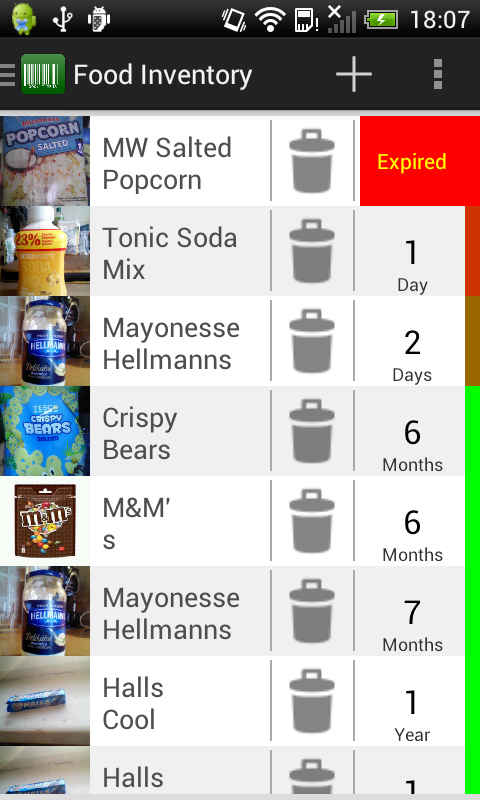
\includegraphics[scale=0.4]{screenshots/app_inventory.png}
  \caption{Inventář}
  \label{fig:AppInventory}
\end{figure}

\clearpage

\subsubsection{Detail inventáře}

Obrazovka~\ref{fig:AppInventoryDetail} zobrazená po stisku položky inventáře ukazuje dialog obsahující detail položky inventáře, kde lze upravit datum spotřeby a případně přejít na detail potraviny, která je položkou tohoto inventáře. Při navigaci zpět zůstává dialog zobrazený stejně jako změny provedené uvnitř.

Tlačítky Ok a Cancel lze uložit či zrušit zvolenou změnu datumu. Uložení způsobí aktualizaci položek inventáře ze serveru.

Samotné načítaní inventáře probíhá za zobrazení standardního ukazatele průběhu, který je schován spolu s~plně načteným inventářem.

\begin{figure}[H]
  \centering
  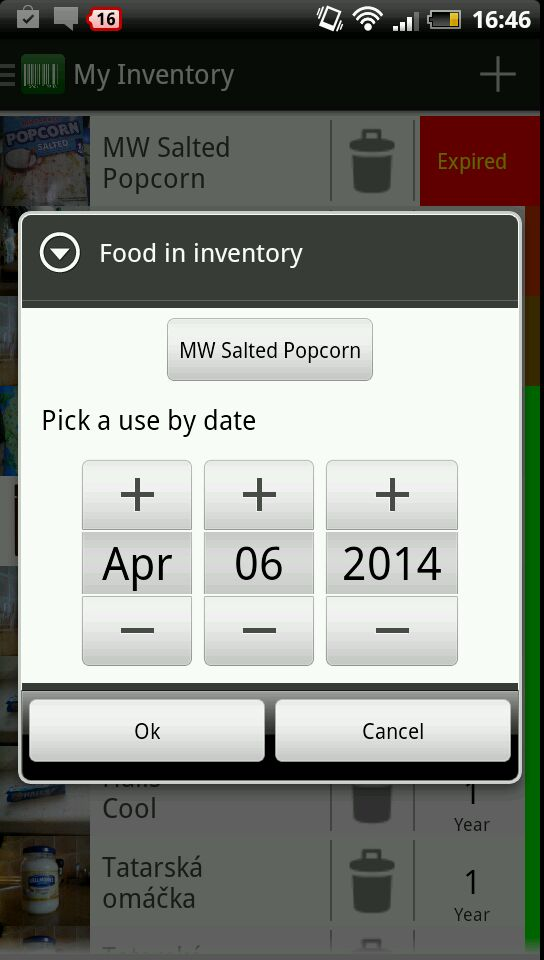
\includegraphics[scale=0.4]{screenshots/app_inventory_detail.jpg}
  \caption{Detail inventáře}
  \label{fig:AppInventoryDetail}
\end{figure}

\clearpage

\subsubsection{Vyhledávání potravin}

Z~menu nebo z~tlačítka přidání v~inventáři se uživatel může dostat do obrazovky vyhledání potravin~\ref{fig:AppSearch}. Pro vyhledávání je zde přítomno jediné textové políčko, které napovídá uživateli, že může vyhledávat pomocí jména potraviny či jejího čárového kódu.

Při psaní textu do políčka vyhledávání je dále zobrazována nápověda jako seznam potravin, které by byly zobrazeny při aktuálním textu v~políčku po stisku klávesy. Pokud uživatel na položku nápovědy klikne, vybraný text se vyplní do políčka.

Pro samotné vyhledání podle políčka stiskne uživatel tlačítko Search, která zobrazí obrazovku~\ref{fig:AppSearchResults}.

V~této obrazovce je do budoucna dále možné uvést filtraci výsledků pomocí jména výrobce, kategorie či jiných parametrů, které jsou již navrženy v~aktuálním databázovém modelu.

\begin{figure}[H]
  \centering
  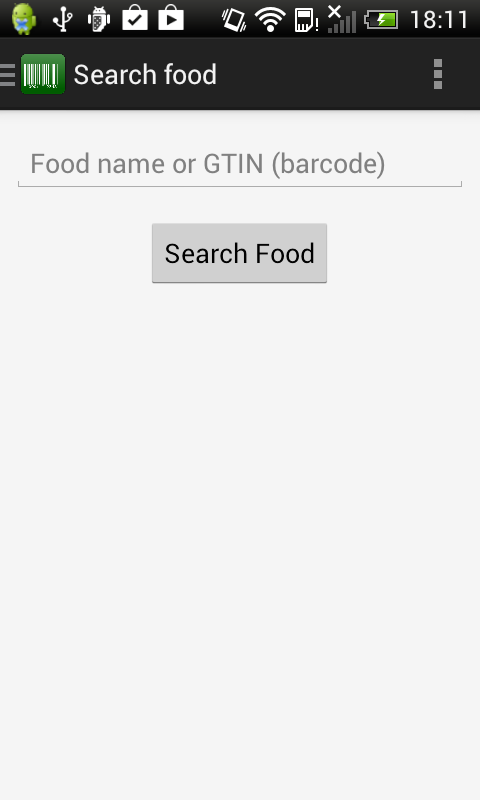
\includegraphics[scale=0.4]{screenshots/app_search.png}
  \caption{Vyhledávání potravin}
  \label{fig:AppSearch}
\end{figure}

\clearpage

\subsubsection{Seznam výsledků hledání potravin}

Tato obrazovka~\ref{fig:AppSearchResults} je zobrazena po vyhledávání v~obrazovce~\ref{fig:AppSearch} a zobrazuje seznam nalezených výsledků. Při probíhajícím vyhledávání je seznam nahrazen prvkem ukazující probíhající činnost, který je zpět schován a zobrazen seznam výsledků při dokončení.

V~tomto seznamu výsledků se v~pravém horním rohu nabízí tlačítko plus, které umožní uživateli přidat novou potravinu, neboť je to místo, kde uživatel zjistí, že takováto potravina neexistuje. Přidání potraviny potom probíha stejně jako při editaci~\ref{fig:AppFoodEdit}.

V~seznamu výsledků je dále možné zobrazit detail potraviny~\ref{fig:AppFoodDetail} nebo přidat potravinu do inventáře stisknutím tlačítka plus, které se nachází vpravo v~položce seznamu. Tím se zobrazí dialog~\ref{fig:AppScanAddFood}.

\begin{figure}[H]
  \centering
  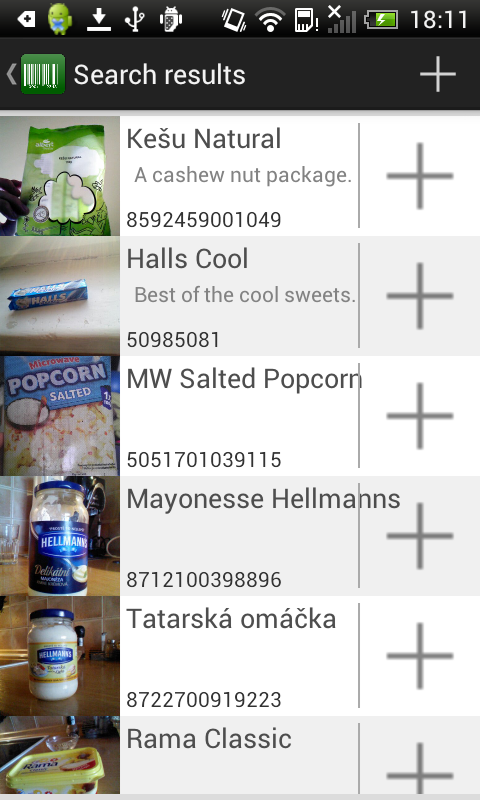
\includegraphics[scale=0.4]{screenshots/app_search_results.png}
  \caption{Seznam výsledků hledání potravin}
  \label{fig:AppSearchResults}
\end{figure}

\clearpage

\subsubsection{Přidání potraviny do inventáře}

V~tomto dialogu~\ref{fig:AppScanAddFood} je zobrazen název potraviny, výběr datumu spotřeby a počet takových kusů. Každý takový kus bude přidán jako jedna položka inventáře.

Stisk tlačítka s~názvem potraviny uživatele přesune do detailu potraviny~\ref{fig:AppFoodDetail}, ze kterého se navigací zpět dostane zpátky do tohoto dialogu.

Tento Dialog se zobrazuje při přidávání z~výsledků hledání potravin i ze čtení čárového kódu za tímto účelem.

\begin{figure}[H]
  \centering
  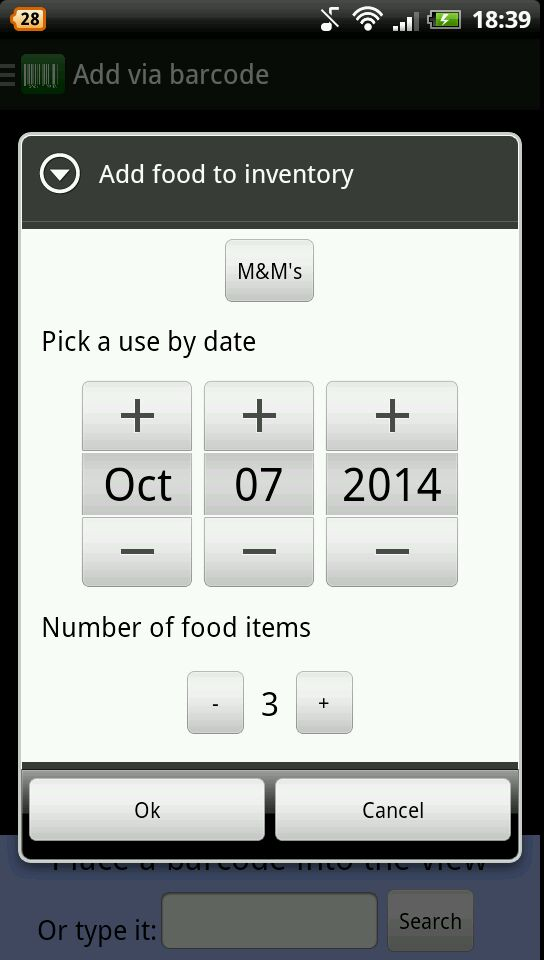
\includegraphics[scale=0.4]{screenshots/app_scan_add_food.jpg}
  \caption{Dialog přidání potraviny do inventáře}
  \label{fig:AppScanAddFood}
\end{figure}

\clearpage

\subsubsection{Detail potraviny}

Obrazovka~\ref{fig:AppFoodDetail} ukazuje částečný detail potraviny. V~tomto místě je možné si potravinu detailnějí prohlédnout a ohodnotit. Také z~této obrazovky lze potravinu upravit pomocí tlačítka tužky v~pravém horním rohu.

Hodnocení potraviny probíha pomocí dialogu, který se dotáže na číselné ohodnocení spolu s~volitelným textem recenze. Pro uložení uživatel stiskne tlačítko Rate, v~opačném případě uživatel stiskne tlačítko Delete, které odstraní hodnocení, pokud existuje. Každý uživatel může potravinu hodnotit maximálně jednou.

Ve spodní části jsou dále vidět 2 uživatelé. První je ten, který potravinu přidal jako první a druhý ten, kdo potravinu naposledny upravil.

\begin{figure}[H]
  \centering
  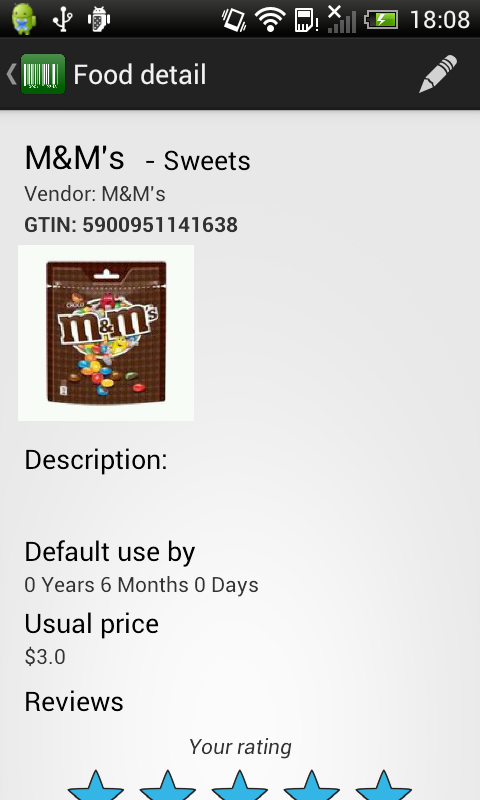
\includegraphics[scale=0.4]{screenshots/app_food_detail.png}
  \caption{Detail potraviny}
  \label{fig:AppFoodDetail}
\end{figure}

\clearpage

\subsubsection{Editace potraviny}

K~editaci potraviny slouží obrazovka~\ref{fig:AppFoodEdit}. Stejně tak slouží i pro přidání potraviny pouze s~tím, že všechny položky jsou nastavené na výchozí hodnoty nebo hodnoty takové, které se podařilo zajistit jiným způsobem. Zde je možné nastavit jméno, výrobce i předem určené obecně uznávané kategorie potravin, čárový kód, obrázky potraviny, hmotnost nebo objem a výchozí datum spotřeby.

Výber kategorie i výrobce poskytuje dialog. Pro výrobce je však možné určit název manuálně, čímž dojde k~přidání výrobce do seznamu všech známých na serveru.

Nastavení čárového kódu je možné buď manuálně, či je vedle něj umístěno tlačítko, které zobrazí stejnou obrazovku jako při přidání potraviny~\ref{fig:AppScanAdd}. Tato obrazovka po načtení čárového kódu zanikne a vyplní číslo čárového kódu tím načteným v předchozí obrazovce.

Obrázky je možné přidávat tlačítkem Add image a mazat pomocí tlačítka Delete již existující obrázky.

Pro samotné uložení změn potraviny (nebo vytvoření nové) slouží tlačítko v~podobě diskety v~pravém horním rohu na panelu ActionBar. Uložení proběhne se zobrazeným dialogem průběhu, neboť nahrávání obrázků může trvat delší dobu.

\begin{figure}[H]
  \centering
  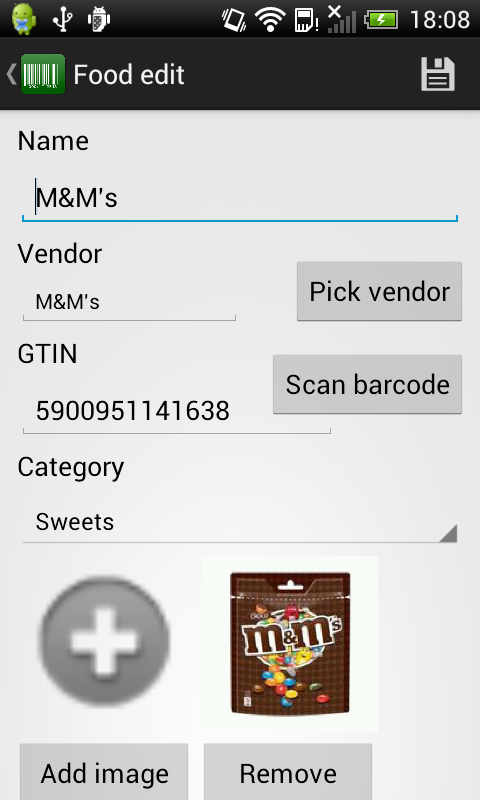
\includegraphics[scale=0.35]{screenshots/app_food_edit.png}
  \caption{Editace potraviny}
  \label{fig:AppFoodEdit}
\end{figure}

\clearpage

\subsubsection{Přidání potraviny do inventáře čárovým kódem}

Pro samotné přidání potraviny pomocí čárového kódu slouží obrazovka~\ref{fig:AppScanAdd}. Uživatel je pobídnut k~umístění čárového kódu do náhledu kamery. Pokud dojde k~úspěšnému načtení, spustí se vyhledání potraviny na serveru, které je signalizováno dialogem pruběhu.

V~případě úspešného nalezení potraviny se zobrazí dialog pro přidání potraviny~\ref{fig:AppScanAdd} stejný jako v~případě manuálního hledání potraviny. Po zrušení dialogu či jeho potvrzení se uživatel vrátí na obrazovku načítaní čárového kódu, aby mohl načíst další potravinu.

Pokud však potravina nalezena nebyla, spustí se dále hledání v~externí databázi, které bude popsáno dále v~této sekci. Signalizováno je také pomocí dialogu průbehu. Při nalezení či nenalezení v~externi databázi se zobrazí dialog, který buď pobízí k vytvoření nové potraviny s~importem nalezených informací~\ref{fig:AppScanAddImport} nebo k~pouhému vytvoření nové potraviny. Do té bude přenesen načtený kód nebo další informace získané z~externí databáze. Přidání potraviny probíhá stejně jako při jejím vytváření při vyhledávání. Po přidání či odmítnutí přidání potraviny se znovu zobrazí obrazovka pro načtení čárového kódu, aby mohl uživatel dále pokračovat v~načítání.

\begin{figure}[H]
  \begin{minipage}{0.5\linewidth} 
    \centering
    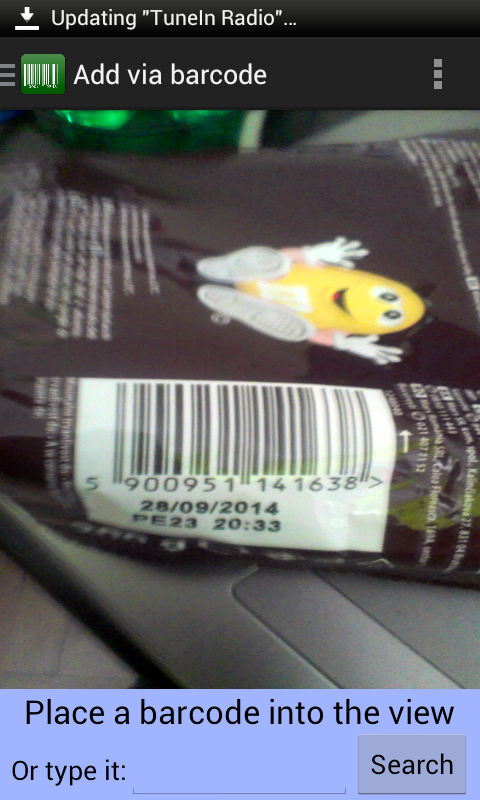
\includegraphics[scale=0.3]{screenshots/app_scan_add.png}
    \caption{Skenování čárového kódu pro přidání potraviny}
    \label{fig:AppScanAdd}
  \end{minipage}
  \begin{minipage}{0.5\linewidth} 
    \centering
    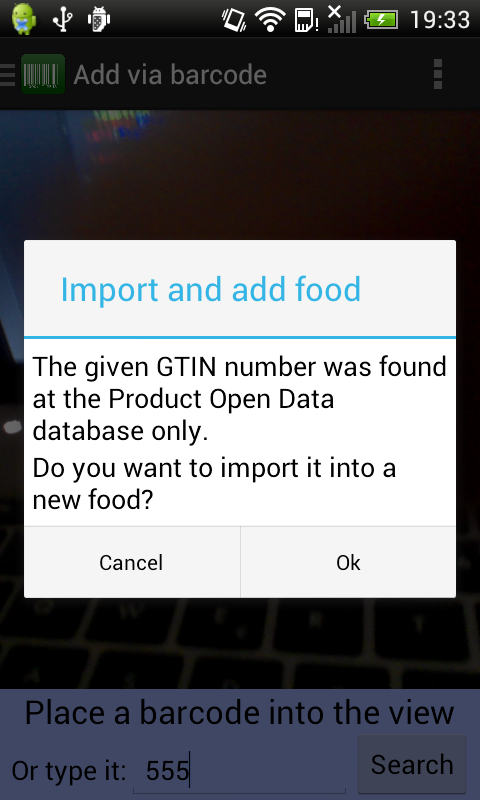
\includegraphics[scale=0.3]{screenshots/app_scan_add_import.png}
    \caption{Import informací z~externí databáze Product Open Data}
    \label{fig:AppScanAddImport}
  \end{minipage} 
\end{figure}

\clearpage

\subsubsection{Odebrání potraviny z~inventáře čárovým kódem}

Podobně jako obrazovka pro načtení čárového kódu pro přidání potraviny~\ref{fig:AppScanAdd} vypadá i tato pro její odebrání z~inventáře.

Při načtení čárového kódu dojde k~vyhledání v~uživatelově inventáři a zobrazení seznamu potravin ~\ref{fig:AppScanRemoveList}, který je stejný jako v obrazovce zobrazení celého inventáře~\ref{fig:AppInventory}. Smazání položky seznamu tedy probíha stejně.

\begin{figure}[H]
  \centering
  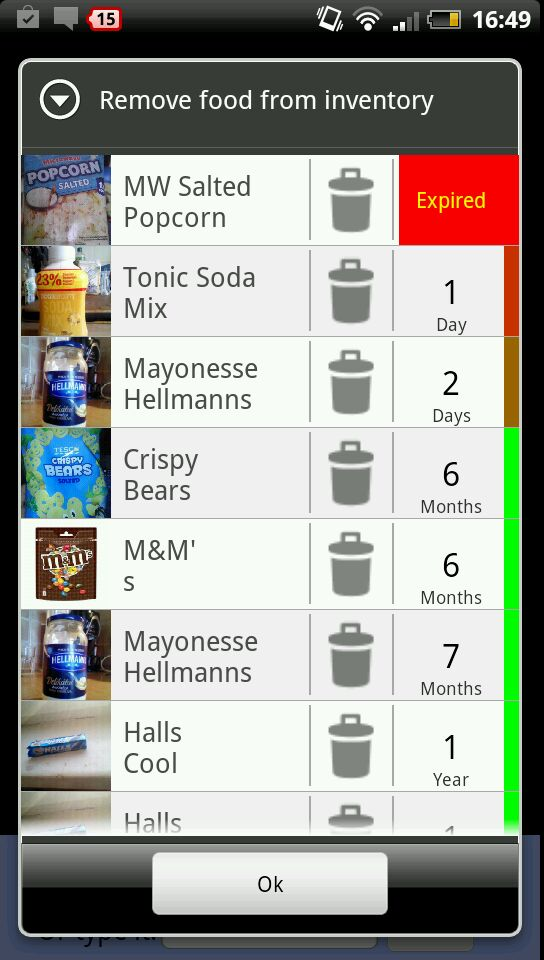
\includegraphics[scale=0.4]{screenshots/app_scan_remove_list.jpg}
  \caption{Seznam nalezených potravin s~daným čárovým kódem}
  \label{fig:AppScanRemoveList}
\end{figure}

\clearpage

\subsubsection{Nastavení}

Pro změnu volitelných vlastností aplikace slouží obrazovka ~\ref{fig:AppInventoryDetail}.

Zde je možné změnit účet uživatele, zakázat stahování obrázků potravin, povolit notifikace a jejich načasování.

Zmíněna je zde také verze spolu s~autorem aplikace.

\begin{figure}[H]
  \centering
  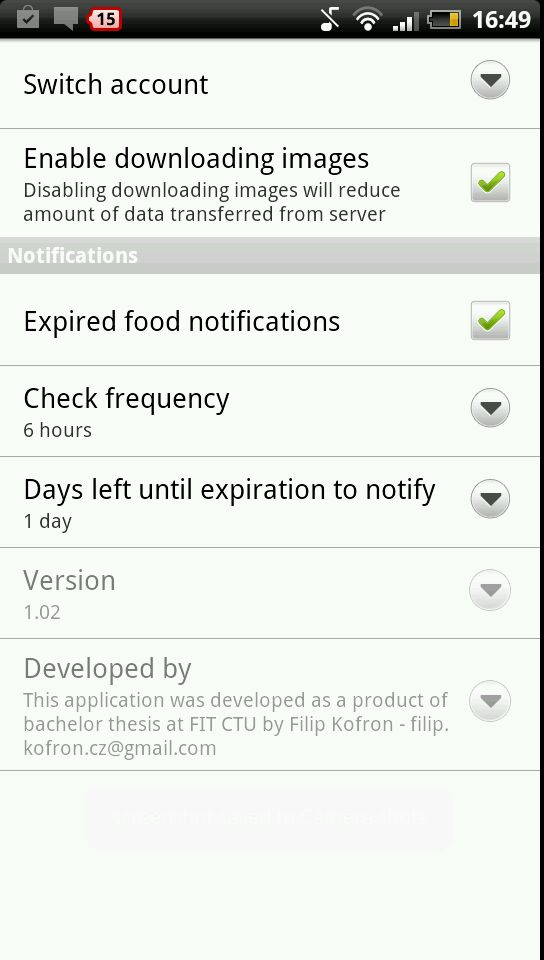
\includegraphics[scale=0.4]{screenshots/app_settings.jpg}
  \caption{Nastavení}
  \label{fig:AppSettings}
\end{figure}

\clearpage

\subsection{Identifikace uživatele}

Uživatel je identifikován pomocí jména, které si vybere při prvním spuštění aplikace nebo z~položky nastavení. Toto jméno je získáno z~účtů uživatele v~jeho zařízení. Použito je pouze takové, které je zároveň splňuje podobu emailové adresy a je tím pádem i unikátní.

Vzhledem k~jednoduchosti aplikace a nízkému nebezpečí zneužití dat uživatele nevyužije aplikace žádné zabezpečení uživatelova účtu. Pokud se však aplikace stane v~budoucnu terčem útoku, bude toto vyžadováno.

\subsection{Vyhledávání čárového kódu v~externí databázi}

Databáze potravin této aplikace bude ze začátku neobsahovat žádné potraviny. Jelikož může být přidání nové potraviny pro uživatele otravné, je vhodné najít cestu, která by zadávání přinejmenším zjednodušila nebo zcela nahradila.

Jednotlivé potraviny výrobců však není jednoduché získat. Díky zaznamenávání potravin pomocí GTIN kódu se však nabízí možnost získat informace o~potravinách z~veřejné a otevřené databáze produktů POD - Product Open Data~\cite{pod}. V~této databázi je možné k~začátku roku 2014 nalézt stovky tisíců záznamů. Informace v~databázi obsahují u~některých potravin složení, ale u~některých naopak pouze jejich výrobce. Možství dat, které se při náhodné analýze této databáze podařilo získat, bylo nedostatečné pro vyplňění většiny potravin. Je zde však možnost využít i pouze částečné informace a ty k~potravině doplňit.

\subsubsection{Připojení k~Product Open Data}

Databázi Product Open Data zpřístupňují online v~době psaní toho textu 3 různé projekty. Jedná se o:
\begin{itemize}
  \item{LSA - http://www.pod.lsa-conso.fr/}
  \item{Mingle IO - https://mingle.io/explore?f=product}
  \item{OpenDataSoft - http://pod.opendatasoft.com/explore/}
\end{itemize}

Projekty Mingle IO a OpenDataSoft spojuje podobné API, se kterým lze komunikovat ve formátu JSON, pomocí kterého se lze dotazovat na čárové kódy všech produktů v~databázi. Projekt LSA je pouze webový vyhledávač.

Mezi OpenDataSoft a Mingle IO nebylo příliš rozdílů, kterými by bylo možné vybrat ten vhodnější. Autor tím pádem zvolil projekt, který se zdál být lépe zdokumentovaný a tím pádem snadnější na implementaci, čímž byl projekt OpenDataSoft.

\subsubsection{Integrace v~aplikaci}

Integrování vyhledávání v~této externí databázi je, jak již bylo zmíněné v~návrhu uživatelského rozhraní, pouze dodatečné vyhledání při nenalezeném produktu, který doplňí podporované informace z~produktu do vytvářené potraviny. U~testovaných potravin v mé domácnosti bylo nalezeno pouze nepatrné množství potravin, u~kterých navíc bylo uvedeno pouze jméno a obrázek. I~takto základní informace však usnadnila přidávání potravin.

\chapter{Implementace}

Tato kapitola popisuje implementaci navrženého serveru a aplikace. Cílem této kapitoly není detailně popsat implementaci, nýbrž snaha popsat vývojové prostředí, zajímavosti a problémy, které se v~průběhu práce vyskytly.

\section{Vývojové nástroje}
V~této sekci lze nalézt všechny použité nástroje při implementaci.

\subsection{Verzovací software a repozitář}

Jelikož byl vývoj uskutečňován na více zařízeních, bylo třeba zajistit vhodné sdílení materiálů a kvůli správě změn také verzování. Jelikož jsem již déle používal software Mercurial~\cite{hg}, usoudil jsem za vhodné, abych pro tuto práci vyzkoušel konkurenční Git~\cite{git} a rozšířil si tak své znalosti. Oba tyto verzovací nástroje si jsou navzájem velmi podobné s~tím rozdílem, že se jen ovládají odlišněji.

Pro sdílení všech materiálů této práce byl zvolen veřejný repozitář pomocí~\cite{repo} služby Github~\cite{github}.

\subsection{Správa a úpravy databáze}

Jako nástroj pro správu databáze byl pro jeho jednoduchost použit řádkový klient dodávaný spolu s~MySQL. Některé úpravy však byli prováděny v~software PhpMyAdmin~\cite{phpmyadmin} v~případech, kdy byl řádkový klient nevhodný či nedostačující. Výhodou PhpMyAdmin je běh z~webového prohlížeče. Bylo tak možné upravovat databázi i bez přístupu k~příkazové řádce.

\subsection{Prostředí pro vývoj klientské aplikace v~OS Android}

Pro tvorbu klienta pro OS Android se jevilo jako vhodné vývojové prostředí Android Studio ~\cite{android_studio}. Tento software umožňuje návrh uživatelského rozhraní a používat známý verzovací software. Díky jeho multiplatformnosti mohl autor aplikaci vyvíjet v~různých operačních systémech.

\subsection{Prostředí pro vývoj serverové aplikace v C++}

Implementace serveru probíhala ve vývojovém prostředí QT Creator~\cite{qtcreator}. Důvod výběru tohoto prostředí byla multiplatformnost a podpora multiplatformního sestavovacího systému CMake~\cite{cmake}, kterým byla popsána celá stromová struktura zdrojového kódu serveru. Díky tomuto lze serverovou aplikaci sestavit na všech rozšířených platformách a vyexportovat případné projektové soubory do dalších vývojových prostředí, které CMake podporuje.

\section{Server}

Jako první částí implementace byl vytvořen základ serveru. Detailní implementace všech částí serveru probíhala průbežně s~aplikací podle požadavků, které kladla funcionalita UI. Výhodou souběžné implementace bylo možné jednodušší přizpůsobení obou stran.

Zdrojový kód byl rozdělen do sekcí, ke kterým byla přiřazena stejnojmenná složka. Tyto sekce jsou sestavovány rekurzivně pomocí zmíněného CMake. Níže jsou jednotlivé sekce popsány. 

\subsection{ConnectedClient}
Název ConnectedClient může být zavádějící, neboť tato sekce ve skutečnosti není klient, ale pouze soubory týkající se spojení s~klientem. Zde dochází k~přijímaní zpráv serveru a k~ošetřování chyb, které mohou nastat při komunikaci s~klientem. Mezi ně patří i chyby ze strany serveru.

Jelikož server používá spoustu vyjímek, je zde pokryto velké množství těch, které lze odchytnout a které by za určitých okolností způsobily pád serveru.

\subsection{Config}
Zde jsou umístěny soubory pro načítání konfigurace a pro jejich získání za běhu serveru. Konfigurace používá formát JSON a při neposkytnutí konfiguračního souboru jsou nastaveny výchozí hodnoty použité pro lokální testování, které server znepřístupňuje veřejnosti.

\subsection{Database}
V~sekci Database jsou implementovány všechny DAO rozhraní, které jsou popsány níže v~podsekci Entity. Jejich implementace využívá třída MySQLManager, která je také umístěna v~této sekci. Jejím úkolem je udržovat již existující a aktuálně nevyužité spojení do databázového serveru, tím recyklovat jejich instance pro další použití novými požadavky klientů. Toto je velmi důležité, neboť připojení na server je časově náročná operace, jak se ukázalo v~průběhu implementace a testování.

\subsection{Entity}
Každá entita doménového modelu vlastní třídu podobného jména obsahující její atributy. Dále jsou zde umístěny všechny rozhraní DAO objektů, které každé entitě přiřazují množinu databázových operací.

\subsection{Handler}
Pro každou zprávu je v~sekci Handler umístěna shodně pojmenovaná obslužná třída, která dle přijaté zprávy dále zpracovává klientské požadavky a sama se postará o~jeho zaslání zpět v~podobě odpovědi.

\subsection{Network}
Soubory síťového socketu serveru a soubory pro uskutečnění odesílání i přijímání dat jsou umístěny v~sekci Network. 

\subsection{Protocol}
Každá zpráva kromě zmíněné zprávy KeepAlive obsahuje požadavek a odpověd. Jejich popis atributy je popsán v~sekci Protocol a také výše v návrhu síťového protokolu.

\subsection{Util}
Pro jednodušší práci s~časovými daty, logování událostí, testování a pro debugování byla vytvořena sekce Util, kde se nalézají také všechny zbylé třídy, které přimo nesouvisí s výše uvedenými sekcemi.

Logování událostí na serveru zde zdůrazním, neboť je velmi důležité sledovat jeho provoz. Tím lze také sesbírat různé informace o pádech a jiných chybách serveru v průběhu testování i při finalním nasazení. Logování bylo zpřístupňeno jako statické metody třídy Log zahrnující výpis chybových, debugovacích a čistě informativních zpráv.

\section{Klient}

Implementace klientské aplikace tvořily dvě části:

\begin{itemize}
	\item{Vytvoření síťové vrstvy, která nezasahovala ještě do návrhu uživatelského rozhraní a sloužila také zároveň k~testování počínající implementace serveru. Byl pro to vytvořen projekt TestClient, který lze nalézt ve zdrojových kódech této práce.}
	\item{Implementace samotné funkcionality UI a napojení síťové vrstvy. Tato část bude níže rozepsána.}
\end{itemize}

\subsection{Struktura zdrojového kódu}

Struktura klientské aplikace je poněkud rozsáhlejší, proto při popisu jednotlivých částí (zde balíků) jsou části přímo spojené s prvky uživatelského rozhraní seskupeny.

Každá část je níže detailněji popsána jako v~případě serveru. Rád bych zde zdůraznil, že tyto části jsou pouze kořenové složky balíku celé aplikace (mimo využité knihovny), a proto ve zdrojovém kódu lze nalézt více podčástí. V~rozsahu této práce není možné popsat každou třídu balíků vzlášť, neboť jich aplikace i server obsahují velmi mnoho. Pro více informací o~každé části je třeba navštívit přímo zdrojový kód.

Při psaní kódu jsem však dbal na zvyklosti při psaní aplikací pro OS Android, které jsem získal vlastních zkušeností.

\subsubsection{Model}

Entity využité v~klientské části aplikace jsou umístěny v~této části.

\subsubsection{Adapter}

Některé části uživatelského rozhraní pro zobrazení dat vyžadují adaptery~\cite{adapter} - třídy, které zprostředkovávají jednotlivé prvky dat, které UI prvky pomocí těchto adapterů přimo získávají a následně je prezentují uživateli. 

Adapterů je v~této aplikaci více, proto jim byla věnována samotná část.

\subsubsection{Network}

Síťová komunikace byla převzata z~projektu TestClient, který byl uveden výše. Stará se o~příjem a odesílání surových dat po síťi, stejně jako vytváření a udržování spojení.

\subsubsection{Protocol}

Požadavky a odpovědi, které tvoří zprávy v~komunikaci, zde mají svou reprezentaci podobně jako v~případě serveru.

\subsubsection{Task}

Každá operace trvající déle či operace, která vyžaduje komunikaci po síti, je potomkem třídy AsyncTask~\cite{async_task} z~Android API. Pomocí implementací potomků této třídy lze jednoduše vytvářet asynchronně probíhající úlohy, jejichž hlavní předností oproti vláknům je zabudovaná synchronizace před spuštěním a po dokončení s~hlavním vláknem, jež je nutné pro přístup k~prvkům UI.

\subsubsection{Barcode}

Třídy využívající knihovnu ZXing, která byla popsána výše, lze nalézt v~této části. Jejich zodpovědnost je pouze dekódování načteného snímku a oznámení výsledku volajícímu.

\subsubsection{Util}

Všechny ostatní třídy, které nezapadají do ostatních částí, lze nalézt zde. Jedná se zejména o~zpracování časových a jiných údajů.

\subsubsection{Cache}

Jelikož jednotlivé potraviny mohou disponovat obrázky, je nutné tyto obrázky uchovávat v~zařízení s~aplikací, aby nedocházelo k~plýtvání přenosu dat po síťi.

\subsubsection{UI prvky - Activity, Fragment, Dialog, Preference, View}

V~této části jsou kategoricky umístěny části prvků UI, které jsou použity ve všech částech klientské aplikace.

Protože jsou tyto prvky v~aplikaci rozšířeny mnohočetně, bylo nutné prvky seskupit podle daných abstraktních tříd. Významy jednotlivých názvů uvedených v~nadpise lze nalézt v~dokumentaci Android API~\cite{android_api}. 

\subsubsection{Background}

Pro průběžné zjišťování stavu trvanlivost potravin bylo nutné zařídit zvláštní část background. Zde lze nalézt registrace událostí pro AlarmManager\cite{alarm_manager}, který způsobí volání těchto operací opakovaně.

Pro získání dat inventáře je zde zjednodušené použití úloh z~části Task, které probíhá oddělěně od zbytku aplikace, která může čí nemusí být v~té době aktivní.

\chapter{Nasazení}

Nasazení probíhalo v~rámci integrace v~průběhu celé implementace.

Server byl nasazen na mém vlastním virtuálním serveru, který běžel již od počátku implementace, abych mohl vyvíjet klientskou aplikaci a testovat ji co nejpřirozeněji. Tento cílový stroj je poháněn Unix-like operačním systémem Linux. Sestavení serveru probíhalo přímo na tomto stroji pomocí CMake. Server byl napojen na lokální databázový software MySQL. 

Pro zálohování dat MySQL databáze jsem vytvořil skript, který je spouštěn pomocí Cron démona každých 6 hodin. Při běhu skriptu dojde ke kompletní záloze celé MySQL databáze na externí ůložiště, odkud lze při ůtoku na aplikaci provést obnovení dat.

Klientská aplikace byla při dokončnování implementace nasazena na Play Store pod názvem Food Inventory - Beta, odkuď si ji mohl jakýkoliv zájemce vlastnící zařízení s~OS Android verze 2.3 a vyšší nainstalovat. Později byla aplikace přejmenována pouze na Food Inventory~\cite{food_inventory_playstore}.

\chapter{Testování}

Každou část aplikace je třeba otestovat, aby byla zajištěna správná funkčnost při nasazení aplikace do produkce. Je tedy nutné testovat server i klientskou aplikaci.

Testování probíhalo ve 3 fázích. První fáze byla zajištěna samotným programátorem (autorem práce) při implementaci. Ta druhá probíhala mezi uživateli, kteří zkoušeli aplikaci v~alfa verzích s~autorovým dozorem. Poslední třetí fáze probíhala před a po dokončení psaní této práce přímo vydáním beta verze aplikace na Play Store.

\section{Testování programátorem}

\subsection{Testování kódu}

Průběh tohoto testování spočíval v~psaní testů nad částmi kódu. Cílem testů bylo ověřit správnost implementace abstraktních tříd a rozhraní v~serverové i klientské aplikaci. Testování bylo shodné s Unit testy, ale pro jednoduchost a nezávislost na dalších knihovnách jsem je napodobil velmi zjednodušeně. Tyto testy jsem vytvářel a aplikoval vždy při vývoji určité části. Testy však nebyly vhodné pro použití jako regresní testy, proto byly ponechány jen po dobu vývoje jednotlivých částí.

\subsection{Testování samotné aplikace}

Další testování programátorem spočívalo v~přímém testování aplikace, čímž bylo ověřena aplikace jako celek a odhaleny zásadní chyby v~implementaci, zejména v~komunikaci protokolem se serverem.

Nejzásadnější chyby, které byly takto odhaleny zahrnovaly překlepy a synchronizační problémy vláken. Všechny tyto chyby bylo možné rychle opravit rovnou při probíhající implementaci a urychlit tak vývoj aplikace i serveru.

\section{Usability testing}

Po dokončení implementace aplikace a otestování aplikace programátorem jsem uskutečnil usability test, který má za úkol zhodnotit celkovou použitelnost aplikace na skupině lidí. Tito lidé byli podrobeni sledovaním při provádění předem daných scénářů, které pokryli běžné činnosti s aplikací a jednotlivé reakce uživatelů byly zaznamenány pro každý scénář. U nich byl také sepsán předpokládaný způsob jejich řešení.

Pro další zisk informací od uživatelů byly položeny níže popsané dotazníky pre-test a post-test.

\subsection{Testovací scénáře a jejich řešení}

Otázky i odpovědi jsou pro pre-test i post-test ve očíslovány stejně.

Otázky pro pre-test zahrnují:
\begin{enumerate}
  \item Jaká je Vaše věková kategorie (v rozmezí desítek let)?
  \item Jaké zařízení s OS Android použijete v testu či jaké zařízení Vám bylo poskytnuto?
  \item Chtěli byste aplikaci s touto funkcionalitou používat?
\end{enumerate}

Otázky pro post-test zahrnují:
\begin{enumerate}
  \item Je pro Vás aplikace srozumitelná?
  \item Zaujala Vás aplikace natolik, že ji budete i nadále používat?
  \item Napadá Vás něco, co byste v aplikaci rádi změnili?
\end{enumerate}

Jednotlivé scénáře jsou očíslované tak, jak jsou níže popsány pozorované reakce a zkušenosti uživatelů při jejich provádění:
\begin{enumerate}
  \item Přidejte Vámi zvolenou potravinu, která není v databázi, pomocí vyhledávání do vašeho inventáře.
    
    \textbf{Předpokládané řešení}: V menu se klikne na tlačítko \textit{Search food}, které uživatele přepne do stejně nazvané aktivity. Zde se vyplní políčko s názvem potraviny. Uživatel stiskne tlačítko \textit{Search}. Jelikož nedojde k nalezení potraviny, je seznam prázdný. V panelu je však tlačítko s ikonou plus, kterým se po stisknutí objeví editace pro přidání nové potraviny. Zde uživatel vyplní údaje o potravině, stisktne tlačítko s ikonou diskety pro uložení. Následně se uživatel pokusí potravinu znovu vyhledat, kde se jit potravina zobrazí a uživatel ji přidá do inventáře přes tlačítko s ikonou plus, které zobrazí dialog s potravinou, kde uživatel vyplní datum spotřeby a potvrdí. Tím je potravina přidána jak v databázi potravin, tak v inventáři uživatele.

  \item Přidejte Vámi zvolenou potravinu, která není v databázi, pomocí skenování čárového kódu do vašeho inventáře.
    
    \textbf{Předpokládané řešení}: V menu se klikne na tlačítko \textit{Add via Barcode}, které uživatele přepne do stejně nazvané aktivity. Zde uživatel načte čárový kód. Jelikož nedojde k nalezení potraviny, zobrazí se dialog pro přidání potraviny (zde se může zobrazit i dialog, že byla potravina nalezena v externí databázi, ale uživatel pokračuje stejně). Po potvrzení, že uživatel chce zadat potravinu, se objeví editace pro přidání nové potraviny. Zde uživatel vyplní chybějící údaje o potravině, stisktne tlačítko s ikonou diskety pro uložení. Následně se zobrazí dialog s potravinou, kterou nalezl po jejím přidání. Dále uživatel pokračuje jako ve scénáři 1.
    
  \item Přidejte Vámi zvolenou potravinu, která už je v databázi, pomocí skenování čárového kódu do vašeho inventáře.
    
    \textbf{Předpokládané řešení}: V menu se klikne na tlačítko \textit{Add via Barcode}, které uživatele přepne do stejně nazvané aktivity. Zde uživatel načte čárový kód. Následně se zobrazí dialog s potravinou, kterou nalezl po jejím přidání. Dále uživatel pokračuje jako ve scénáři 1.
  
  \item Odeberte Vámi zvolenou potravinu, která už je v inventáři, pomocí skenování čárového kódu.
    
    \textbf{Předpokládané řešení}: V menu se klikne na tlačítko \textit{Remove via Barcode}, které uživatele přepne do stejně nazvané aktivity. Zde uživatel načte čárový kód. Následně se zobrazí dialog se seznamem potravin, které se shodují s načteným čárovým kódem. Uživatel stiskne tlačítko s ikonou koše. Tím je potravina odebrána z inventáře uživatele.
  
  \item Odeberte Vámi zvolenou potravinu, která už je v inventáři, při prohlížení vašeho inventáře.
    
    \textbf{Předpokládané řešení}: Pokud ještě uživatel není v intentáři, pak v menu klikne na tlačítko \textit{My Inventory}, které uživatele přepne do stejně nazvané aktivity. Zde se zobrazí seznam všech potravin v inventáři. Uživatel pokračuje stejně jako ve scénáři 4.
  
  \item Vámi zvolenou potravinu, která už je v databázi, vyhledejte a upravte nějaký údaj. Jako například upravte výchozí datum spotřeby.
    
    \textbf{Předpokládané řešení}: V menu se klikne na tlačítko \textit{Search food}, které uživatele přepne do stejně nazvané aktivity. Zde se vyplní políčko s názvem potraviny. Po stisku hledat se zobrazí seznam potravin se shodujícím se názvem. Zde uživatel klikne na potravinu. Tím se dostane do detailu potraviny, kde stiskne ikonu tužky, která ho zavede do editace. Zde změní údaj, potravinu uloží stiskem tlačitka s ikonou diskety. Následně se tím vrátí do detailu, kde má být údaj aktualizován na upravený.
  
\end{enumerate}

\subsection{Provádení testu}

\subsubsection{Testovací subjekt 1}

Odpovědi pre-test:

\begin{enumerate}
  \item 40-50 let
  \item Huawei M886
  \item Ano.
\end{enumerate}

Jednotlivé úkoly:
\begin{enumerate}
  \item V tomto úkolu se uživateli podařilo dosáhnout řešení přesně podle daného scénáře, uživatel však vykazoval mírné známky zmatení z prázdného seznamu, přesto však včas uvážil možnost stisknutí tlačítka s ikonou plus, které bylo správný cíl.
  \item V tomto úkolu se uživateli podařilo dosáhnout řešení, uživatel si však stěžoval, že musel čárový kód potraviny načíst znovu, aby ji mohl následně přidat i do inventáře.
  \item V tomto úkolu se uživateli podařilo dosáhnout řešení přesně podle daného scénáře.
  \item V tomto úkolu se uživateli podařilo dosáhnout řešení, načítání kódu ale trvalo mnohem déle než v předchozím testu. Toto uživatele na chvíli negativně rozrušilo.
  \item V tomto úkolu se uživateli podařilo dosáhnout řešení přesně podle daného scénáře.
  \item V tomto úkolu se uživateli podařilo dosáhnout řešení přesně podle daného scénáře.
\end{enumerate}

Odpovědi pro post-test:
\begin{enumerate}
  \item Ano, ale pro začátek by bylo vhodné v aplikaci uvést nějaký návod.
  \item Pokud v aplikaci zařídíte, aby se nemusela potravina znovu načítat po přidání, pak ano.
  \item Vše co jsem zmínila.
\end{enumerate}

\subsubsection{Testovací subjekt 2}

Odpovědi pre-test:

\begin{enumerate}
  \item 50-60 let
  \item Xperia sola
  \item Ano.
\end{enumerate}

Jednotlivé úkoly:
\begin{enumerate}
  \item V tomto úkolu byl uživatel zmatený, zběsile klikal v inventáři místo toho, aby klikl na menu. Dále byl uživatel zmatený při zadání výchozího data spotřeby. Myslel si totiž, že to je již datum spotřeby té dané potraviny.
  \item V tomto úkolu se uživateli podařilo dosáhnout řešení přesně podle daného scénáře.
  \item V tomto úkolu se uživateli podařilo dosáhnout řešení přesně podle daného scénáře.
  \item V tomto úkolu se uživateli podařilo dosáhnout řešení přesně podle daného scénáře.
  \item V tomto úkolu se uživateli podařilo dosáhnout řešení přesně podle daného scénáře.
  \item V tomto úkolu se uživateli podařilo dosáhnout řešení přesně podle daného scénáře.
\end{enumerate}

Odpovědi pro post-test:
\begin{enumerate}
  \item Nyní již ano.
  \item Ještě si to rozmyslím.
  \item Chtělo by zjednodušit zadávání výchozího data spotřeby a nějak to zdůraznit.
\end{enumerate}

\subsubsection{Testovací subjekt 3}

Odpovědi pre-test:

\begin{enumerate}
  \item 20-30 let
  \item Huawei G700
  \item Určitě ano.
\end{enumerate}

Jednotlivé úkoly:
\begin{enumerate}
  \item V tomto úkolu se uživateli podařilo dosáhnout řešení přesně podle daného scénáře. Při přidávání potraviny však uživatel nenašel výrobce potraviny a znejistil. Potravinu však i tak přidal.
  \item V tomto úkolu se uživateli podařilo dosáhnout řešení. Po přidání potraviny ale uživatel stiskl tlačítko zpět, které ukončilo aplikaci. Uživatel byl znepokojen a výrazně dal najevo nespokojenost s tímto chováním aplikace. Uživatel totiž předpokládal, že po přidání potraviny se znovu objeví inventář, ze kterého uživatel začal přidávat potravinu.
  \item V tomto úkolu se uživateli podařilo dosáhnout řešení přesně podle daného scénáře.
  \item Uživatel se v tomto úkolu spletl a místo odebíraní se pokusil potravinu přidat. Poté však již nalezl správné tlačítko v menu. Při načtení a nalezení potraviny uživatele zmátlo, že dialog s potravinou disponuje tlačítkem \textit{Ok}, které ve skutečnosti slouží pouze ke schování dialogu. Toto tlačítko by však podle uživatele mělo být nazváno spíše \textit{Cancel}. Poté již potravinu odebral.
  \item Uživatel v tomto úkolu kliknul těsně vedle tlačítka s ikonou koše. Tím se zobrazil detail potraviny v inventáři. Po druhé již vše proběhlo podle předpokládaného řešení.
  \item V tomto úkolu se uživateli podařilo dosáhnout řešení přesně podle daného scénáře.
\end{enumerate}

Odpovědi pro post-test:
\begin{enumerate}
  \item Ano.
  \item Ano.
  \item Pouze bych přidala možnost, aby se potravina nenačítala zbytečně dvakrát, když už jsem ji jednou načetla.
\end{enumerate}

\subsubsection{Testovací subjekt 4}

Odpovědi pre-test:

\begin{enumerate}
  \item 20-30 let
  \item Nexus 5
  \item Ne.
\end{enumerate}

Jednotlivé úkoly:
\begin{enumerate}
  \item V tomto úkolu se uživateli podařilo dosáhnout řešení přesně podle daného scénáře.
  \item V tomto úkolu se uživateli podařilo dosáhnout řešení přesně podle daného scénáře. Při naskenování čárového kódu uživatel předpokládal, že ho zpět vrátí do inventáře, stejně jako u testovacího subjektu 4. Uživateli se tedy podařilo aplikaci omylem ukončit.
  \item V tomto úkolu se uživateli podařilo dosáhnout řešení přesně podle daného scénáře.
  \item V tomto úkolu se uživateli podařilo dosáhnout řešení přesně podle daného scénáře.
  \item V tomto úkolu se uživateli podařilo dosáhnout řešení přesně podle daného scénáře.
  \item V tomto úkolu se aplikace ukončila kvůli chybě spojení se serverem. Chybu zřejmě způsobil mobilní internet, který měl v té chvíli slabý signál. Druhý pokus se již však zadařil.
\end{enumerate}

Odpovědi pro post-test:
\begin{enumerate}
  \item Aplikace by se neměla zabíjet kvůli stisknutí zpět při skenováni, ale měla by mě dostat zpátky do inventáře. Jinak ano.
  \item Ne, nemám zájem. Nápad je to ovšem zajímavý a aplikace dělá to, co má.
  \item Už jsem to zmínil.
\end{enumerate}

\subsubsection{Testovací subjekt 5}

Odpovědi pre-test:

\begin{enumerate}
  \item 20-30 let
  \item Nexus 4
  \item Ne.
\end{enumerate}

V testu číslo jedna byl uživatel ve věkové kategorii 20-30 let s mobilním telefonem Nexus 4.

Jednotlivé úkoly:
\begin{enumerate}
  \item V tomto úkolu se uživateli podařilo dosáhnout řešení, ale trvalo mu déle, než nalezl tu správnou cestu. Aplikaci nejdříve celou prozkoumal a až poté splnil úkol.
  \item V tomto úkolu se uživateli nepodařilo na první pokus dosáhnout řešení, neboť nebylo možné načíst čárový kód potraviny. Druhý pokus se podařil jen díky tomu, že uživatel potravinu nenačetl pomocí kamery, ale zadal čárový kód ručně.
  \item V tomto úkolu se uživateli podařilo dosáhnout řešení podobně jako v předchozím úkolu.
  \item Při plnění tohoto úkolu došlo k restartování mobilního telefonu. Stalo se tak v momentě, kdy se zobrazila virtuální klávesnice na obrazovce, která posunula ostatní prvky skenovací obrazovky výše. Chybu bylo možné zreprodukovat.
  \item V tomto úkolu se uživateli podařilo dosáhnout řešení přesně podle daného scénáře.
  \item V tomto úkolu se uživateli podařilo dosáhnout řešení přesně podle daného scénáře.
\end{enumerate}


Odpovědi pro post-test:
\begin{enumerate}
  \item Na začátku jsem si nebyl jistý tím, jak vůbec něco přidat, ale teď už mi to je jasné a je to jednoduché.
  \item Jedině když aplikace nebude padat.
  \item Zpravit pády v aplikaci a možná vylepšit tu čtečku čárových kódů.
\end{enumerate}

\subsection{Souhrn výsledků testu}

Zásadní nedostatky, které byly objeveny v tomto testu jsou:
\begin{itemize}
	\item{Pro přidání potraviny pomocí načítání čárového kódu je nutné jej znovu načíst, aby jej bylo možné přidat i do inventáře.}
	\item{Aplikace by si měla pamatovat kroky zpět v navigaci, které nevedou přímo z menu. Problém se objevil u dialogu v intentáři, kde je možné zvolit způsob přidání potraviny, který uživatele přesune na vybranou obrazovku stejně jako navigace na tyto místa z menu. Problém pak nastane, když se uživatel chce vrátit zpět do inventáře. Místo toho se totiž aplikace ukončí.}
	\item{Při prvním používaní jsou uživatelé zmateni. Je nutné zajistit nápovědy v prázdném inventáři nebo ve vyhledávání potravin, pokud není žádná potravina nalezena.}
\end{itemize}

\section{Testování vydáním na Play Store}

Vydáním beta verze aplikace na Play Store byla plně naimplementovaná aplikace testována přímo samotnými uživateli. V~době psaní této práce se tohoto testování zúčastnilo 5 osob různých věkových kategorií.

Průběh tohoto testování záležel na samotných uživatelích. Uživatelé měli možnost se k~aplikaci vyjádřit na přání autora.

Při tomto testování byly do doby psaní tohoto textu objeveny tyto nedostatky:

\begin{itemize}
	\item{Nemožnost zvolit kameru, která je použita pro snímání potravin. Některé mobilní telefony totiž mají zadní i přední snímací čip obrazu a někteří uživatelé vyjádřili touhu po této funkcionalitě. Výchozí totiž byla pouze zadní kamera, jelikož obvykle mívá vyšší rozlišení. V případě, že nebyla zadní kamera dostupná, byla vybrána další dostupná.}
	\item{Zasekávání kamery. Tato chyba vzniká při uspání aktivity pro skenování čárového kódu a následném probuzení.}
	\item{Samovolné uspání zařízení z~neaktivity uživatele. Stává se tak obvykle při delším neúspěšném skenování čárového kódu potraviny.}
\end{itemize}

Opravení těchto nedostatků již proběhne mimo rámec této práce.

\begin{conclusion}
Cílem této práce bylo najít možné řešení celosvětového problému plýtvání potravin v~podobě mobilní aplikace na platformě Android. Řešení bylo nutné nejdříve zanalyzovat a získat tak požadavky, které musí aplikace splňovat. Poté byla navrhnuta aplikace, která všechny požadavky splňovala.
	
Výsledkem práce vznikla aplikace, která řeší část tohoto problému evidencí potravin. Rámec aplikace obsahuje jednoduchou klientskou aplikaci pro platformu Android a serverovou aplikaci, která byla naimplementována pomocí multiplatformních knihoven v~jazyce C++, který měl za cíl efektivně využít slabé prostředky stroje, na němž byl server nasazen.

Celá aplikace byla po dobu vývoje i následně po něm dostupná veřejně ve formě zdrojových kódů na veřejném repozitáři webové služby Github~\cite{repo}. Při tvorbě aplikace byly využity svobodné i open-source nástroje a open-source knihovny, tím pádem i tato aplikace byla vydána jako open-source.

V~době psaní tohoto textu je aplikace nasazena v~testovací beta verzi již veřejně dostupná každému k~vyzkoušení.

\section{Budoucí vývoj}

Aplikace, která vznikla v~rámci této práce, má mnoho nedostatků. Zde se pokusím popsat ty, které lze do budoucna vyřešit.

\subsection{Knihovna pro čtení čárových kódů}
Jedním z~nich je nedokonalost knihovny ZXing, která čtení čárových sice zvládá, ale testováním uživateli vyšlo najevo, že ne dostatečně. Do budoucna by tedy bylo vhodné zvážit i jiné svobodné či komerční řešení nebo vyvinout vlastní řešení založeném na jiném algoritmu, který by umožňoval načítaní čárových kódu potravin spolehlivěji.

\subsection{Zabezpečení aplikace a komunikace}
Na zabezpečení dat uživatelů této aplikace není kladen žádný důraz. Účty různých lidí lze jendoduše přidat do OS Android účtů a přistoupit tak neoprávněně na účet jiných lidí. Stejně tak není šifrované spojení mezi klientem a serverem.

Pokud by mělo být zabezpečení v budoucnu zvýšeno, pak by bylo nutné upravit zprávy tak, aby jejich obsah byl dostatečně zašifrovaný. Také uživatelské účty by bylo nutné chránit heslem. Tyto změny by však nebyly nijak zásadní a celkem snadno by je bylo možné aplikovat.

Otevřenost aplikace uživatelům nabízí spoustu způsobů, jak na aplikaci zaútočit. Bylo by vhodné vyvinout pro aplikaci sledovací mechanismy, které by detekovaly nevhodné chování uživatelů při editacích čí pridavaní potravin.

\subsection{Zálohování}
Zálohování na serveru zatím probíhá pouze jako záloha celé databáze.

Při nasazení se však ukázalo, že by bylo vhodné mít možnost vrátit potravinu do původního stavu po útoku nějakým škodolibým uživatelem bez vracení celé databáze do určitého stavu v minulosti.

Toto zálohování by mohlo být vytvořeno jako 1 ku N vztah, potravina ku její historii. Poté by bylo možné historii uživatelům přímo nabízet k prohlednutí, případně k navrácení do aktualní potraviny. Také by se tímto daly navrátit škody detekované například automaticky jako spam nebo souvislé poškozování potravin.

\subsection{UI}
Uživatelské rozhraní klientské aplikace je další velkou nedokonalostí. Ačkoliv bylo vytvořeno co nejjednodušeji pro přehlednost a rychlost zároveň, není toto rozhraní příliš příjemné, neboť využívá strohý výchozí styl platformy OS Android. V~budoucnu by bylo možné pro aplikaci získat lepší styl a zpříjemnit tak celou aplikaci. Zároveň by tak mohla být i přitažlivější při výberu uživateli.

\subsection{Výkon serverového stroje}
Další nedostatek je v~cílovém stroji na nasazení serveru. Pokud by aplikace měla v~budoucnu být využívána mnoho uživateli, pak by bylo nutné zajistit pro běh serveru výkonější stroj.

\subsection{Rozšíření na další platformy}
Jelikož platformu Android nevlastní všichni uživatelé, bylo by vhodné vyvinout pro aplikaci také webovou verzi, která by byla dostupná i na jiných zařízeních, které nedisponují operačním systémem Android.

\end{conclusion}

\bibliographystyle{csn690}
\bibliography{mybibliographyfile}

\appendix

\chapter{Seznam použitých zkratek}
% \printglossaries
\begin{description}
	\item[API] Application Programming Interface
	\item[DAO] Data Access Object
	\item[GTIN] Global Trade Item Number
	\item[HTML] HyperText Markup Language
	\item[JSON] JavaScript Object Notation
	\item[NDK] Native Development Kit
	\item[OS] Operační systém
	\item[SDK] Software Development Kit
	\item[UI] User Interface
	\item[VM] Virtual Machine
	\item[XML] Extensible Markup Language
\end{description}

% % % % % % % % % % % % % % % % % % % % % % % % % % % % 
% % Tuto kapitolu z výsledné práce ODSTRAŇTE.
% % % % % % % % % % % % % % % % % % % % % % % % % % % % 
% 
% \chapter{Návod k~použití této šablony}
% 
% Tento dokument slouží jako základ pro napsání závěrečné práce na Fakultě informačních technologií ČVUT v~Praze.
% 
% \section{Výběr základu}
% 
% Vyberte si šablonu podle druhu práce (bakalářská, diplomová), jazyka (čeština, angličtina) a kódování (ASCII, \mbox{UTF-8}, \mbox{ISO-8859-2} neboli latin2 a nebo \mbox{Windows-1250}). 
% 
% V~české variantě naleznete šablony v~souborech pojmenovaných ve formátu práce\_kódování.tex. Typ může být:
% \begin{description}
% 	\item[BP] bakalářská práce,
% 	\item[DP] diplomová (magisterská) práce.
% \end{description}
% Kódování, ve kterém chcete psát, může být:
% \begin{description}
% 	\item[UTF-8] kódování Unicode,
% 	\item[ISO-8859-2] latin2,
% 	\item[Windows-1250] znaková sada 1250 Windows.
% \end{description}
% V~případě nejistoty ohledně kódování doporučujeme následující postup:
% \begin{enumerate}
% 	\item Otevřete šablony pro kódování UTF-8 v~editoru prostého textu, který chcete pro psaní práce použít -- pokud můžete texty s~diakritikou normálně přečíst, použijte tuto šablonu.
% 	\item V~opačném případě postupujte dále podle toho, jaký operační systém používáte:
% 	\begin{itemize}
% 		\item v~případě Windows použijte šablonu pro kódování \mbox{Windows-1250},
% 		\item jinak zkuste použít šablonu pro kódování \mbox{ISO-8859-2}.
% 	\end{itemize}
% \end{enumerate}
% 
% 
% V~anglické variantě jsou šablony pojmenované podle typu práce, možnosti jsou:
% \begin{description}
% 	\item[bachelors] bakalářská práce,
% 	\item[masters] diplomová (magisterská) práce.
% \end{description}
% 
% \section{Použití šablony}
% 
% Šablona je určena pro zpracování systémem \LaTeXe{}. Text je možné psát v~textovém editoru jako prostý text, lze však také využít specializovaný editor pro \LaTeX{}, např. Kile.
% 
% Pro získání tisknutelného výstupu z~takto vytvořeného souboru použijte příkaz \verb|pdflatex|, kterému předáte cestu k~souboru jako parametr. Vhodný editor pro \LaTeX{} toto udělá za Vás. \verb|pdfcslatex| ani \verb|cslatex| \emph{nebudou} s~těmito šablonami fungovat.
% 
% Více informací o~použití systému \LaTeX{} najdete např. v~\cite{wikilatex}.
% 
% \subsection{Typografie}
% 
% Při psaní dodržujte typografické konvence zvoleného jazyka. České \uv{uvozovky} zapisujte použitím příkazu \verb|\uv|, kterému v~parametru předáte text, jenž má být v~uvozovkách. Anglické otevírací uvozovky se v~\LaTeX{}u zadávají jako dva zpětné apostrofy, uzavírací uvozovky jako dva apostrofy. Často chybně uváděný symbol "{} (palce) nemá s~uvozovkami nic společného.
% 
% Dále je třeba zabránit zalomení řádky mezi některými slovy, v~češtině např. za jednopísmennými předložkami a spojkami (vyjma \uv{a}). To docílíte vložením pružné nezalomitelné mezery -- znakem \texttt{\textasciitilde}. V~tomto případě to není třeba dělat ručně, lze použít program \verb|vlna|.
% 
% Více o~typografii viz \cite{kobltypo}.
% 
% \subsection{Obrázky}
% 
% Pro umožnění vkládání obrázků je vhodné použít balíček \verb|graphicx|, samotné vložení se provede příkazem \verb|\includegraphics|. Takto je možné vkládat obrázky ve formátu PDF, PNG a JPEG jestliže používáte pdf\LaTeX{} nebo ve formátu EPS jestliže používáte \LaTeX{}. Doporučujeme preferovat vektorové obrázky před rastrovými (vyjma fotografií).
% 
% \subsubsection{Získání vhodného formátu}
% 
% Pro získání vektorových formátů PDF nebo EPS z~jiných lze použít některý z~vektorových grafických editorů. Pro převod rastrového obrázku na vektorový lze použít rasterizaci, kterou mnohé editory zvládají (např. Inkscape). Pro konverze lze použít též nástroje pro dávkové zpracování běžně dodávané s~\LaTeX{}em, např. \verb|epstopdf|.
% 
% \subsubsection{Plovoucí prostředí}
% 
% Příkazem \verb|\includegraphics| lze obrázky vkládat přímo, doporučujeme však použít plovoucí prostředí, konkrétně \verb|figure|. Například obrázek \ref{fig:float} byl vložen tímto způsobem. Vůbec přitom nevadí, když je obrázek umístěn jinde, než bylo původně zamýšleno -- je tomu tak hlavně kvůli dodržení typografických konvencí. Namísto vynucování konkrétní pozice obrázku doporučujeme používat odkazování z~textu (dvojice příkazů \verb|\label| a \verb|\ref|).
% 
% \begin{figure}\centering
% 	
\includegraphics[width=0.5\textwidth, angle=30]{cvut-logo-bw}
% 	\caption[Příklad obrázku]{Ukázkový obrázek v~plovoucím prostředí}\label{fig:float}
% \end{figure}
% 
% \subsubsection{Verze obrázků}
% 
% % Gnuplot BW i barevně
% Může se hodit mít více verzí stejného obrázku, např. pro barevný či černobílý tisk a nebo pro prezentaci. S~pomocí některých nástrojů na generování grafiky je to snadné.
% 
% Máte-li například graf vytvořený v programu Gnuplot, můžete jeho černobílou variantu (viz obr. \ref{fig:gnuplot-bw}) vytvořit parametrem \verb|monochrome dashed| příkazu \verb|set term|. Barevnou variantu (viz obr. \ref{fig:gnuplot-col}) vhodnou na prezentace lze vytvořit parametrem \verb|colour solid|.
% 
% \begin{figure}\centering
% 	\includegraphics{gnuplot-bw}
% 	\caption{Černobílá varianta obrázku generovaného programem Gnuplot}\label{fig:gnuplot-bw}
% \end{figure}
% 
% \begin{figure}\centering
% 	\includegraphics{gnuplot-col}
% 	\caption{Barevná varianta obrázku generovaného programem Gnuplot}\label{fig:gnuplot-col}
% \end{figure}
% 
% 
% \subsection{Tabulky}
% 
% Tabulky lze zadávat různě, např. v~prostředí \verb|tabular|, avšak pro jejich vkládání platí to samé, co pro obrázky -- použijte plovoucí prostředí, v~tomto případě \verb|table|. Například tabulka \ref{tab:matematika} byla vložena tímto způsobem.
% 
% \begin{table}\centering
% 	\caption[Příklad tabulky]{Zadávání matematiky}\label{tab:matematika}
% 	\begin{tabular}{|l|l|c|c|}\hline
% 		Typ		& Prostředí		& \LaTeX{}ovská zkratka	& \TeX{}ovská zkratka	\tabularnewline \hline \hline
% 		Text		& \verb|math|		& \verb|\(...\)|	& \verb|$...$|		\tabularnewline \hline
% 		Displayed	& \verb|displaymath|	& \verb|\[...\]|	& \verb|$$...$$|	\tabularnewline \hline
% 	\end{tabular}
% \end{table}
% 
% % % % % % % % % % % % % % % % % % % % % % % % % % % % 

\chapter{Obsah přiloženého CD}

%upravte podle skutecnosti

\begin{figure}
	\dirtree{%
		.1 readme.txt\DTcomment{stručný popis obsahu CD}.
		.1 build.
		.2 Thesis.pdf\DTcomment{text práce ve formátu PDF}.
		.2 Client.apk\DTcomment{instalovatelná aplikace pro OS Android}.
		.1 src\DTcomment{zdrojové kódy práce}.
		.1 db.
		.2 model.mwb\DTcomment{databázový model ve formátu MySQL Workbench}.
		.2 create.sql\DTcomment{skript vytvořející strukturu databáze ve formátu SQL}.
		.1 doc\DTcomment{zdrojová forma práce ve formátu \LaTeX{}}.
	}
\end{figure}

\end{document}
